\clearpage
\section{Extended Related Work}
\label{extended_related_works}

\paragraph{Parallel reasoning and test-time scaling.}
Test-time scaling approaches fall into two paradigms: sequential methods such as long chain-of-thought that iteratively refine a single solution \citep{madaan2023selfrefine}, and parallel methods that generate multiple reasoning paths simultaneously \citep{DBLP:journals/corr/abs-2110-14168, setlur2025scalingtesttimecomputeverification,
pan2025learning, zhao2025samplescrutinizescaleeffective, singhi2025whentosolve, lian2025threadweaveradaptivethreadingefficient}. Parallel scaling helps explore diverse solution paths simultaneously; however, it requires effective mechanisms to combine various solutions. For math, majority voting is effective due to objective answers \citep{wang2023selfconsistency, snell2024scalingllmtesttimecompute, wu2025inferencescalinglawsempirical}, but this approach is domain-specific and unavailable for domains such as code generation and scientific discovery, where answers are not directly comparable to each other via exact matching. For code generation, prior work \citep{li2025stesttimescaling} has explored test-time scaling but requires executable test cases in the evaluation data or generated by larger models like GPT-4 for clustering and selection, while $\mu$Code \citep{jain2025multiturn} leverages external, multi-turn execution feedback, both of which are specific to code generation.
We focus on \textit{self-verification} for parallel reasoners, where a model judges its own generations without external verified or feedback.

\paragraph{Self-verification and self-aggregation}
Early work by \citet{weng2023selfverification} demonstrated that LLMs can verify their own chain-of-thought reasoning, improving accuracy on arithmetic and commonsense tasks. Related to this, there have been multiple studies analysing the self-refinement capabilities and limitations of LLMs \citep{madaan2023selfrefine, stechly2025on, huang2024large}, however, they focus on a sequential reasoning setting, while our focus is on explicit self-verification in parallel reasoning. Recently \citet{lu2025doesverificationpayoff} show that LLMs exhibit a bias toward accepting incorrect solutions during pointwise self-verification. On the other hand, self-aggregation methods like RSA \citep{venkatraman2025recursiveselfaggregationunlocksdeep} and parallel-distill-refine \citep{madaan2025rethinkingthinkingtokensllms} combine solutions generated by the same model, but suffer from diversity collapse (Section~\ref{sec:swiss_pairwise_verification}), resulting in correct solutions being discarded during inference. Such aggregation-based approaches are orthogonal to self-verification and can be combined with better self-verification for more better performance and efficient test-time scaling. Our work addresses limitations of the above prior work by studying pairwise self-verification in a parallel reasoning setup, showing it significantly outperforms pointwise self-verification while preserving solution diversity.

\paragraph{Generative verifiers and reward models.}
Reward models have been central to LLM alignment and RLHF \citep{christiano2017rlhf, ziegler2019rlhf, DBLP:journals/corr/abs-2009-01325}, and have emerged as a natural mechanism for scoring and selecting LLM generations \citep{DBLP:journals/corr/abs-2110-14168, DBLP:conf/nips/ZhengC00WZL0LXZ23}. Recent work demonstrates that generative reward models, which produce chain-of-thought reasoning before scoring, substantially outperform discriminative approaches \citep{mahan2024generative, zhang2025generativeverifiersrewardmodeling, shi2025heimdalltesttimescalinggenerative, saha2025learningplanreason}, with RL-trained verifiers showing improved judgment performance \citep{liu2025inferencetimescalinggeneralistreward, whitehouse2025j1incentivizingthinkingllmasajudge}.
Recognizing that pairwise comparison is often easier than absolute scoring, several works have explored pairwise reward models: PairRM \citep{jiang2023llmblender} trains a discriminative pairwise ranker for ensembling LLM outputs, while GenSelect \citep{toshniwal2025genselect} and concurrent work by \citet{mahdavi2025scaling} scale generative verification for mathematical reasoning. Related to this, \citet{zhao2025majority} propose AggLM, which trains an aggregator via RL to synthesize correct answers for improving majority voting.
However, these approaches use \textit{separate} verifiers or aggregator models. Our work differs in two key aspects: (1) we study \textit{self}-verification, where the same parallel reasoner model judges its own outputs. This eliminates the need for additional training with curated judge data, saves memory, and reduces the computational overhead associated with external verification. (2) We co-train the model to be both a solution generator and a pairwise self-verifier in a unified framework.

\paragraph{Co-training for generation and verification.}
Training separate verifiers incurs significant overhead in compute, memory, and data curation. Recent work has explored co-training a single model for both generation and verification. \citet{sareen2025puttingvaluerlbetter} train models to self-verify online during RL, ensuring the verifier sees in-distribution generations and uses this capability to perform better majority voting at test-time for math reasoning. \citet{liu2025trustverifyselfverificationapproach} extends this to unified CoT verifiers, while \citet{zha2025rltangoreinforcinggenerator} co-trains a separate process reward model that provides intermediate rewards. Offline approaches train verifiers or aggregators on data sampled from the base model \citep{venkatraman2025recursiveselfaggregationunlocksdeep, ruan2025critiquecoderenhancingcodermodels}. For code generation specifically, several works co-train generators with unit-test producers \citep{wang2025coevolvingllmcoderunit, lee2025learninggenerateunittest}. However, existing co-training methods rely on \textit{pointwise} verification rewards. Our \method{}-PairRL framework instead co-trains for \textit{pairwise} self-verification in an online, co-evolving setup, which we show yields superior test-time scaling performance.

\section{\method{}-PointRL Training Details}
\label{sec:appendix-pointwise-training}

To provide a fair comparison for our pairwise verification approach, we train \method{}-PointRL using the same co-evolving setup as \method{}-PairRL. The key difference lies in the verification objective: instead of comparing pairs of solutions, \method{}-PointRL assigns an independent score to each solution.

\textbf{Verification Reward.} For pointwise verification, the model evaluates a single solution $s$ and outputs a confidence score between 1-10 which is normalized to $v \in [0, 1]$. The reward is computed as:
\begin{equation}
    r_{\text{verif}} = \mathbb{I}(|v - y| \leq 0.2) \cdot (1 - |v - y|)
\end{equation}
where $y \in \{0, 1\}$ is the ground truth correctness. The sparsity threshold prevents the ``safe bet'' collapse mode where the model learns to always output $v = 0.5$ (in practice, not applying the sparsity threshold leads to collapse in solution generation performance and is necessary for stable training).

\textbf{Training Configuration.} All hyperparameters (learning rate, batch size, rollout allocation, etc.) are identical to \method{}-PairRL as shown in Table~\ref{tab:training_hyperparams}. The only difference is the verification prompt and reward computation.

\textbf{Inference.} At inference time, \method{}-PointRL generates $N$ solutions and independently scores each one. The solution with the highest pointwise score is selected as the final answer.


\section{Hyperparameters}
\label{sec:appendix_hyperparams}

\subsection{Inference Sampling Parameters}
\label{sec:appendix_inference_hyperparams}

\textbf{Inference Framework.} We use SGLang~\citep{zheng2024sglangefficientexecutionstructured} for all inference experiments, which provides efficient batched inference for large language models.

\textbf{Sampling Parameters.} We set temperature $T=0.6$ for all code generation experiments and $T=1.0$ for all math reasoning experiments to encourage better exploration of the solution space. We use top-p sampling with $p=0.95$ for all experiments. For experiments with \pairinfer{} in Section~\ref{sec:swiss_pairwise_verification} where we test the inference algorithm on widely used open source LLMs like GPT-OSS-20B, GPT-OSS-120B, Qwen3-4B-Instruct-2507, Qwen3-4B-Thinking-2507, we set the max generation length to 32768 for all methods.

For trained model evaluations in Section~\ref{sec:unified_rl} we find that training all models lead to longer chains of thoughts, as is commonly the case in RLVR \citep{deepseekai2025deepseekr1incentivizingreasoningcapability}. This leads to frequent truncation, especially for the baseline RL model. To resolve this, we adopt the truncate-and-continue-generation method from prior work \citep{yang2025qwen3technicalreport, sareen2025puttingvaluerlbetter}. When generation reaches the maximum token budget (\texttt{finish\_reason=length}), we resume decoding by appending the partially generated assistant output to the message history and issuing a continuation request. If the truncated output does not contain a closing \texttt{</thinking>} tag, we append the following transition sentence before continuing: \emph{``Considering the limited time by the user, I have to directly give the required response based on the reasoning till now directly.\texttt{</thinking>}''}. This explicitly closes the thinking block and forces the continuation to produce the final answer. If the truncated output already contains \texttt{</thinking>}, we directly continue generation without appending any additional text. We continue the generation for 2K tokens, making the total maximum generation length 34 K for all experiments in Section \ref{sec:unified_rl}.


\textbf{Number of Samples.} We generate $N \in \{8, 16\}$ candidate solutions for most experiments. For budget-matched comparisons between pointwise and pairwise verification, we additionally evaluate pointwise verification with $N=32$ samples to match the total LLM calls of pairwise verification with $N=16$ and budget 3$\times$. This budget-matched comparison is performed only for GPT-OSS-20B and Qwen3-4B-Instruct models.

\textbf{Verification Budget.} For \pairinfer{} experiments in Section~4, we evaluate verification budgets of 1$\times$, 2$\times$, and 3$\times$ the number of base solutions ($N$). Full results across all budgets are provided in the appendix figures.

\textbf{Experimental Runs.} All inference experiments for base models (Section~4) are run once. All trained model results (Section~5) are run 3 times with different random seeds, and we report the mean. Due to the computational cost of running multiple seeds, we limit the budget exploration for trained models to 1$\times$ and 2$\times$, though we believe performance can further scale with additional budget for the pairwise method (\pairinfer{}).

\textbf{Swiss Refinement Algorithm Parameters.} For \pairinfer{}, we use the following settings: Minimum degree $d_{\min} = 2$ (each solution compared at least twice in coverage phase), Swiss window size $h = 8$, Confidence floor set to a small value, $\tau = 0.1$ for weighted aggregation. We do not tune parameters to any specific benchmark. We use the same parameters across benchmarks or models across all experiments.

\subsection{Training Hyperparameters}

Table~\ref{tab:training_hyperparams} summarizes the key training hyperparameters. We train models using rLLM \citep{rllm2025} and verl \citep{sheng2024hybridflow} backend.

\begin{table}[h]
\centering
\caption{Training hyperparameters for \method{}.}
\label{tab:training_hyperparams}
\begin{tabular}{lc}
\toprule
\textbf{Hyperparameter} & \textbf{Qwen3-4B-Inst} \\
\midrule
Learning rate & $1 \times 10^{-6}$ \\
Batch size & 64 \\
Rollouts per prompt ($G$) & 4 (8 for baseline RL) \\
Judge rollouts & 4 (0 for baseline RL) \\
Max prompt length & 10240 \\
Max response length & 24576 \\
Temperature & 0.6 \\
Top-p & 0.95 \\
Clip ratio (low) & 0.2 \\
Clip ratio (high) & 0.28 \\
$\lambda$ (loss weight) & 1.0 \\
KL coefficient & 0 \\
Entropy coefficient & 0 \\
Std normalization & No \\
Loss aggregation & token-mean \\
\bottomrule
\end{tabular}
\end{table}


\begin{figure}[htbp]
    \centering
    \setlength{\tabcolsep}{3pt}
    \renewcommand{\arraystretch}{1.0}

    \begin{tabular}{ccc}
        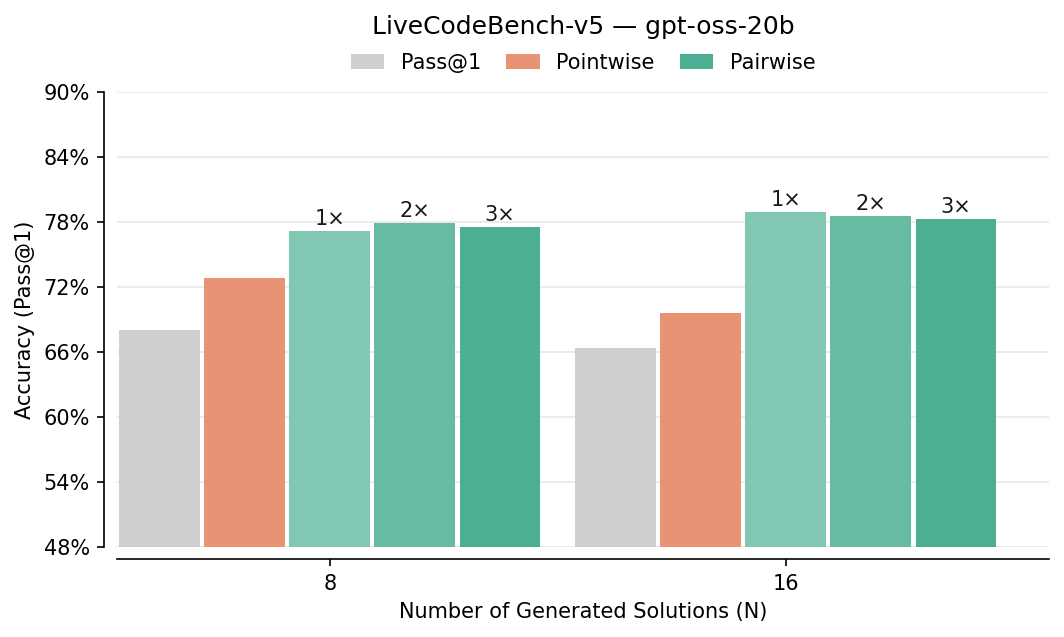
\includegraphics[width=0.32\textwidth]{images_verif/LiveCodeBench-v5-gpt-oss-20b.png} &
        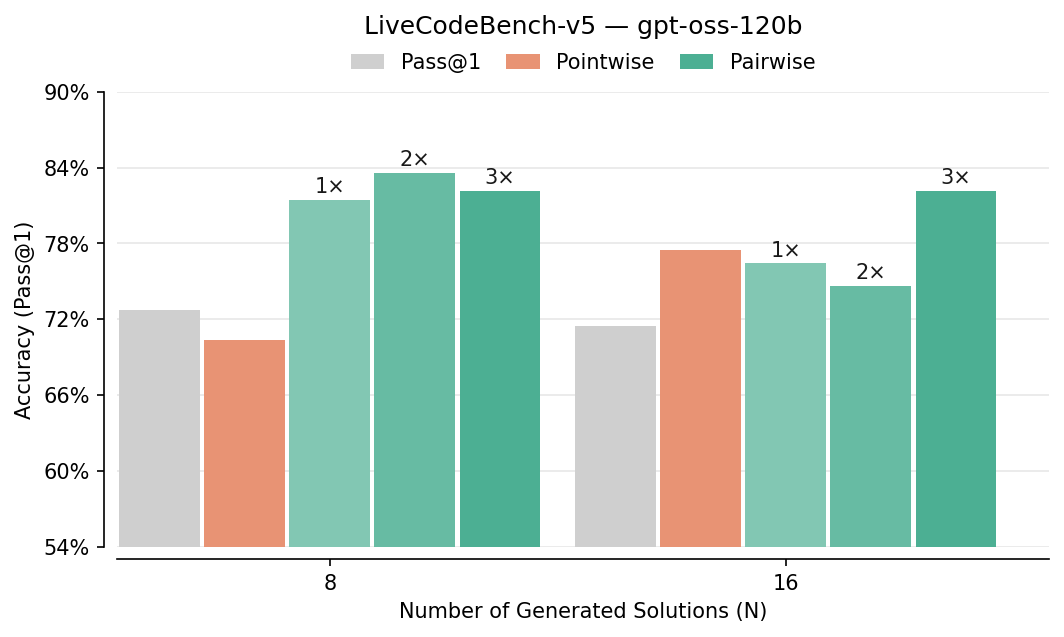
\includegraphics[width=0.32\textwidth]{images_verif/LiveCodeBench-v5-gpt-oss-120b.png} &
        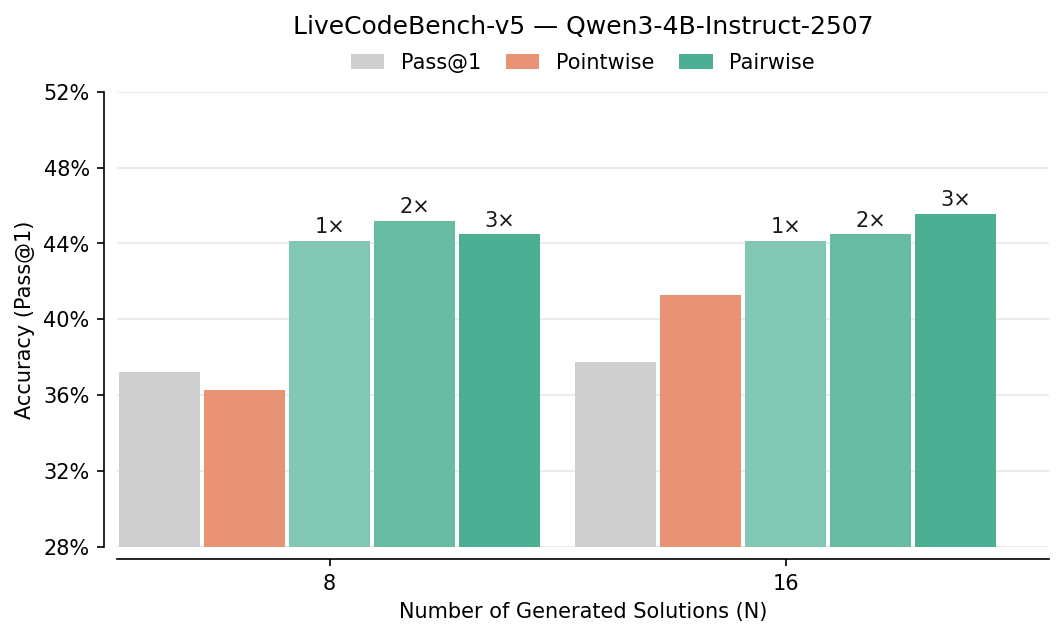
\includegraphics[width=0.32\textwidth]{images_verif/LiveCodeBench-v5-Qwen3-4B-Instruct-2507.png} \\
        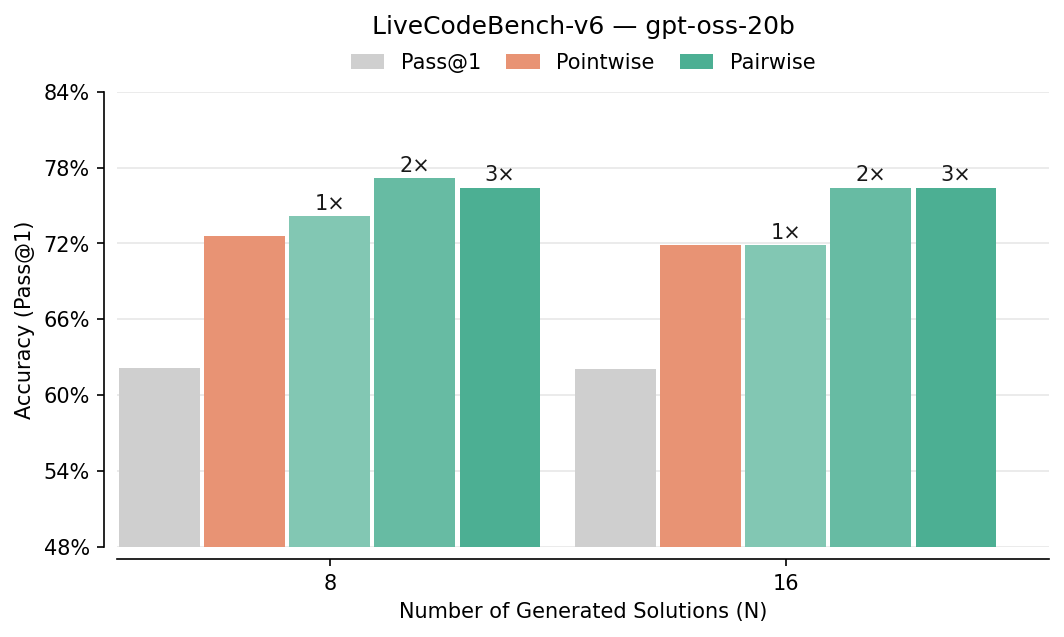
\includegraphics[width=0.32\textwidth]{images_verif/LiveCodeBench-v6-gpt-oss-20b.png} &
        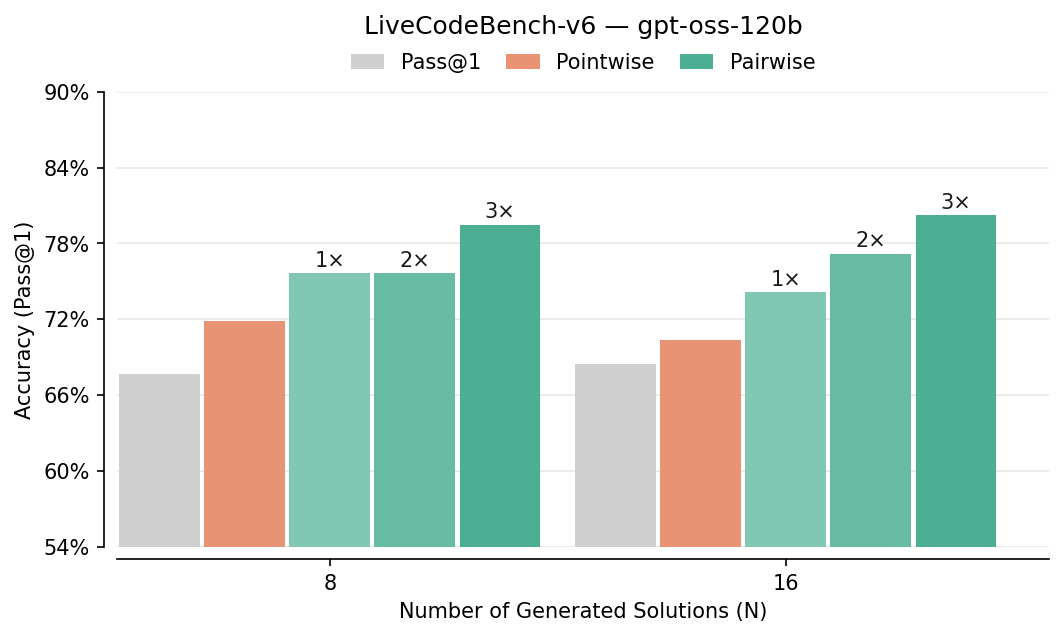
\includegraphics[width=0.32\textwidth]{images_verif/LiveCodeBench-v6-gpt-oss-120b.png} &
        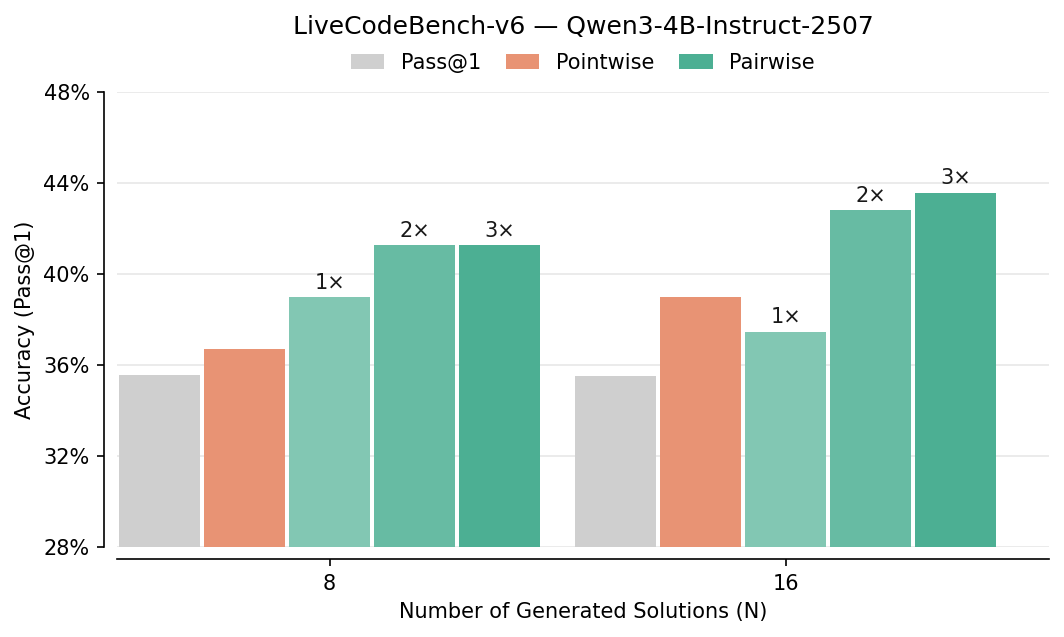
\includegraphics[width=0.32\textwidth]{images_verif/LiveCodeBench-v6-Qwen3-4B-Instruct-2507.png} \\
        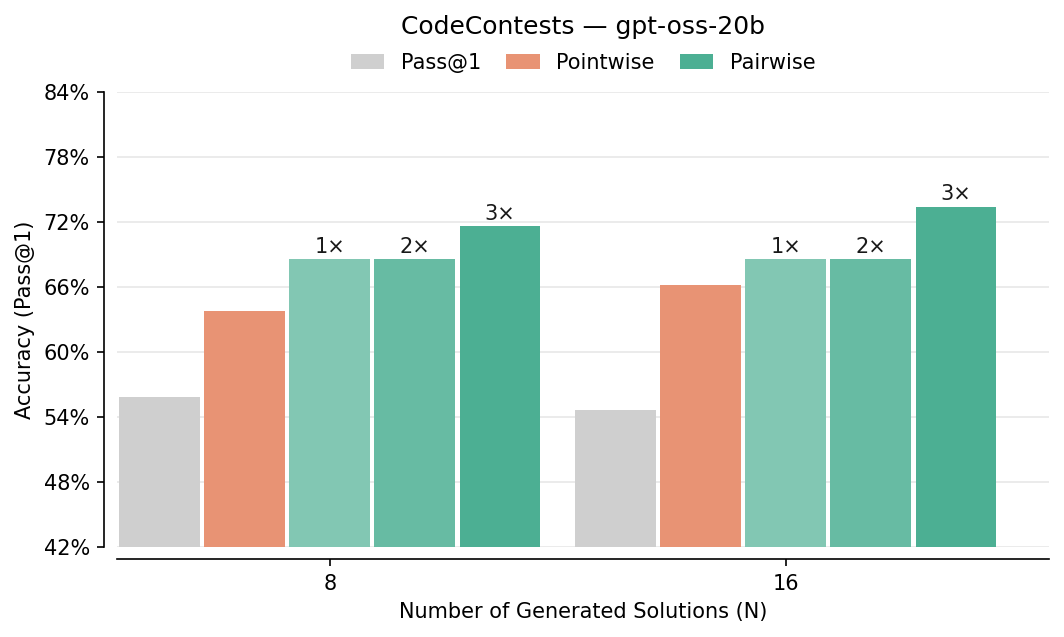
\includegraphics[width=0.32\textwidth]{images_verif/CodeContests-gpt-oss-20b.png} &
        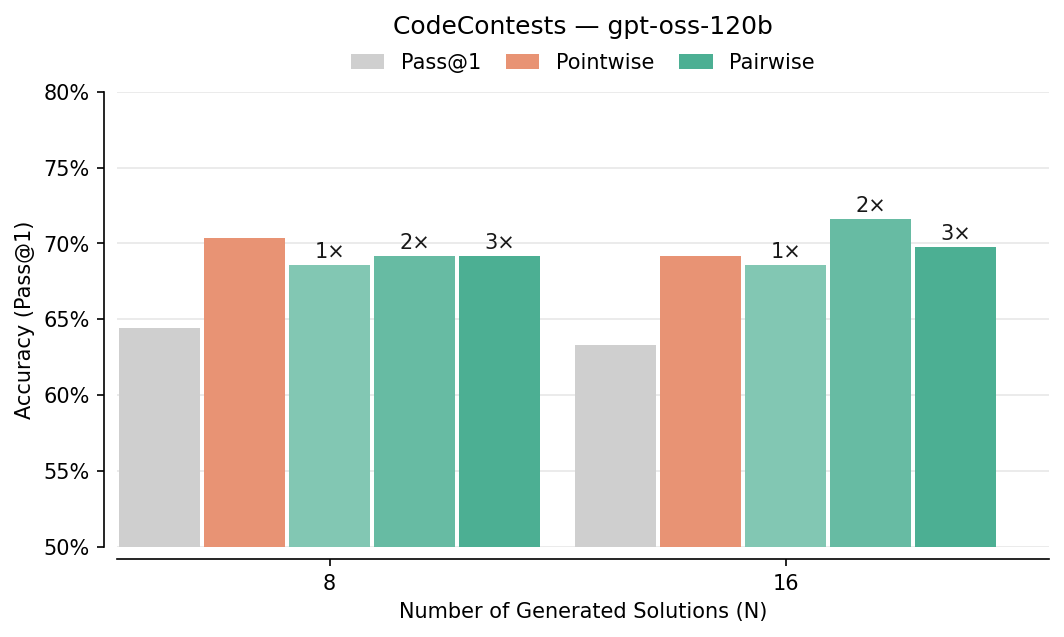
\includegraphics[width=0.32\textwidth]{images_verif/CodeContests-gpt-oss-120b.png} &
        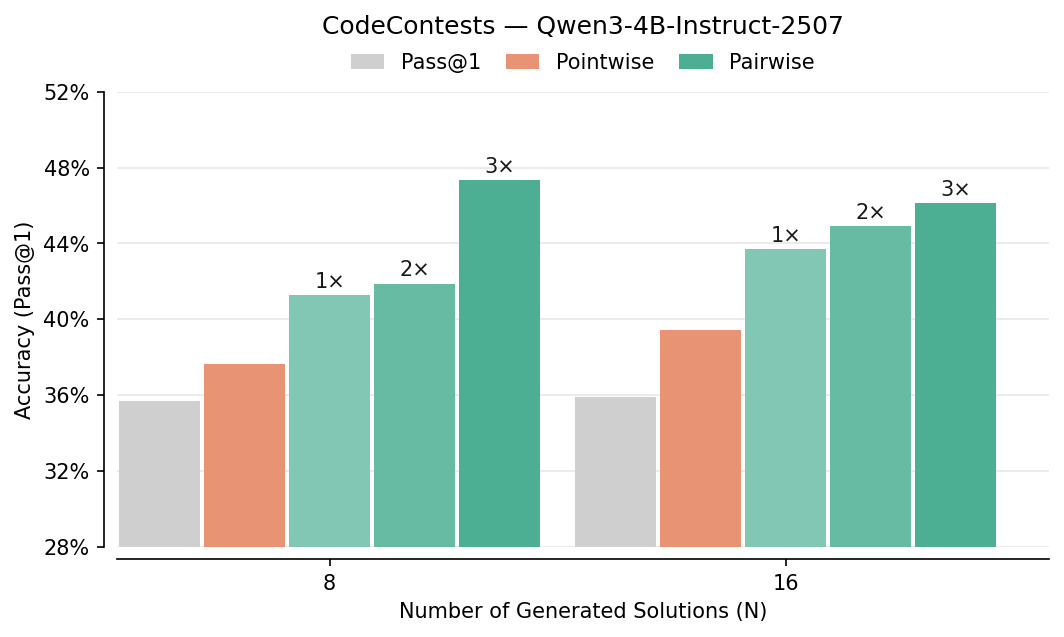
\includegraphics[width=0.32\textwidth]{images_verif/CodeContests-Qwen3-4B-Instruct-2507.png} \\
        \multicolumn{3}{c}{
            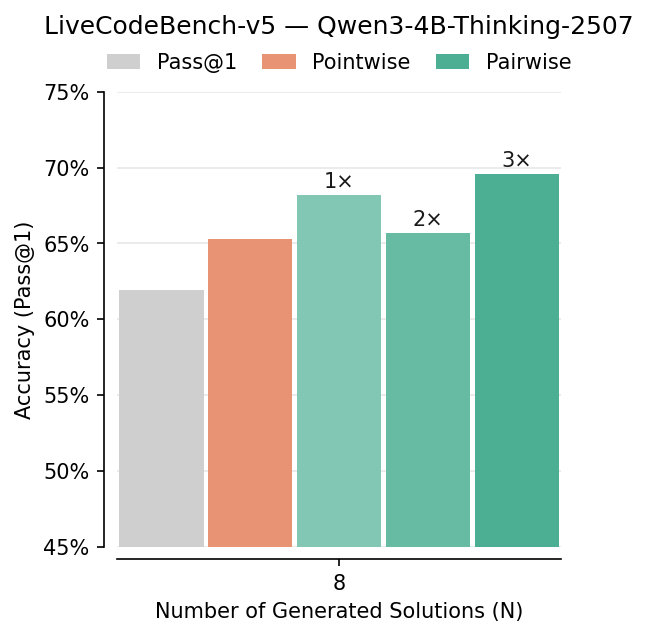
\includegraphics[width=0.25\textwidth]{images_verif/LiveCodeBench-v5-Qwen3-4B-Thinking-2507.png}
            \hspace{0.02\textwidth}
            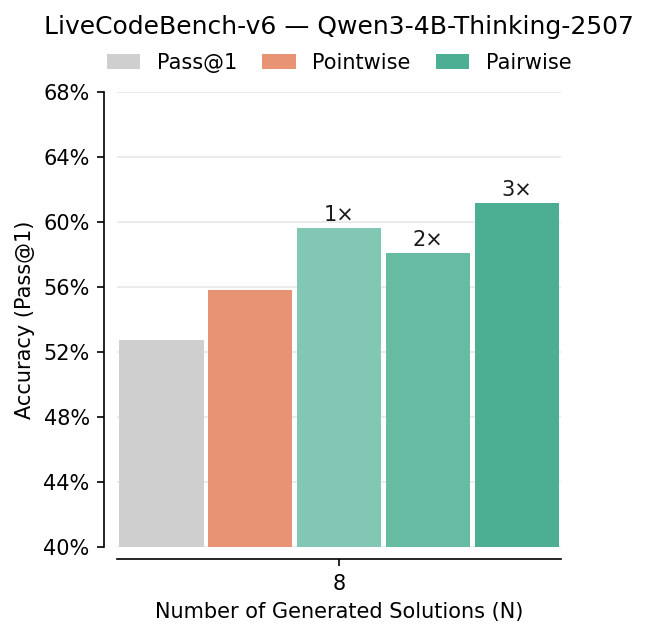
\includegraphics[width=0.25\textwidth]{images_verif/LiveCodeBench-v6-Qwen3-4B-Thinking-2507.png}
        } \\
    \end{tabular}

    \caption{Self-verification bar plots across benchmarks and models (LiveCodeBench-v5, LiveCodeBench-v6, and CodeContests).
        Each plot compares Pass@1, pointwise verification, and pairwise verification (budgets 1$\times$/2$\times$/3$\times$) at $N\in\{8,16\}$.
        For Qwen3-4B-Thinking (bottom row), we run experiments only on LiveCodeBench at $N=8$ to manage compute.
    }
    \label{fig:appendix-all-verif-bars}
\end{figure}


\clearpage

\begin{figure}[t]
  \centering
  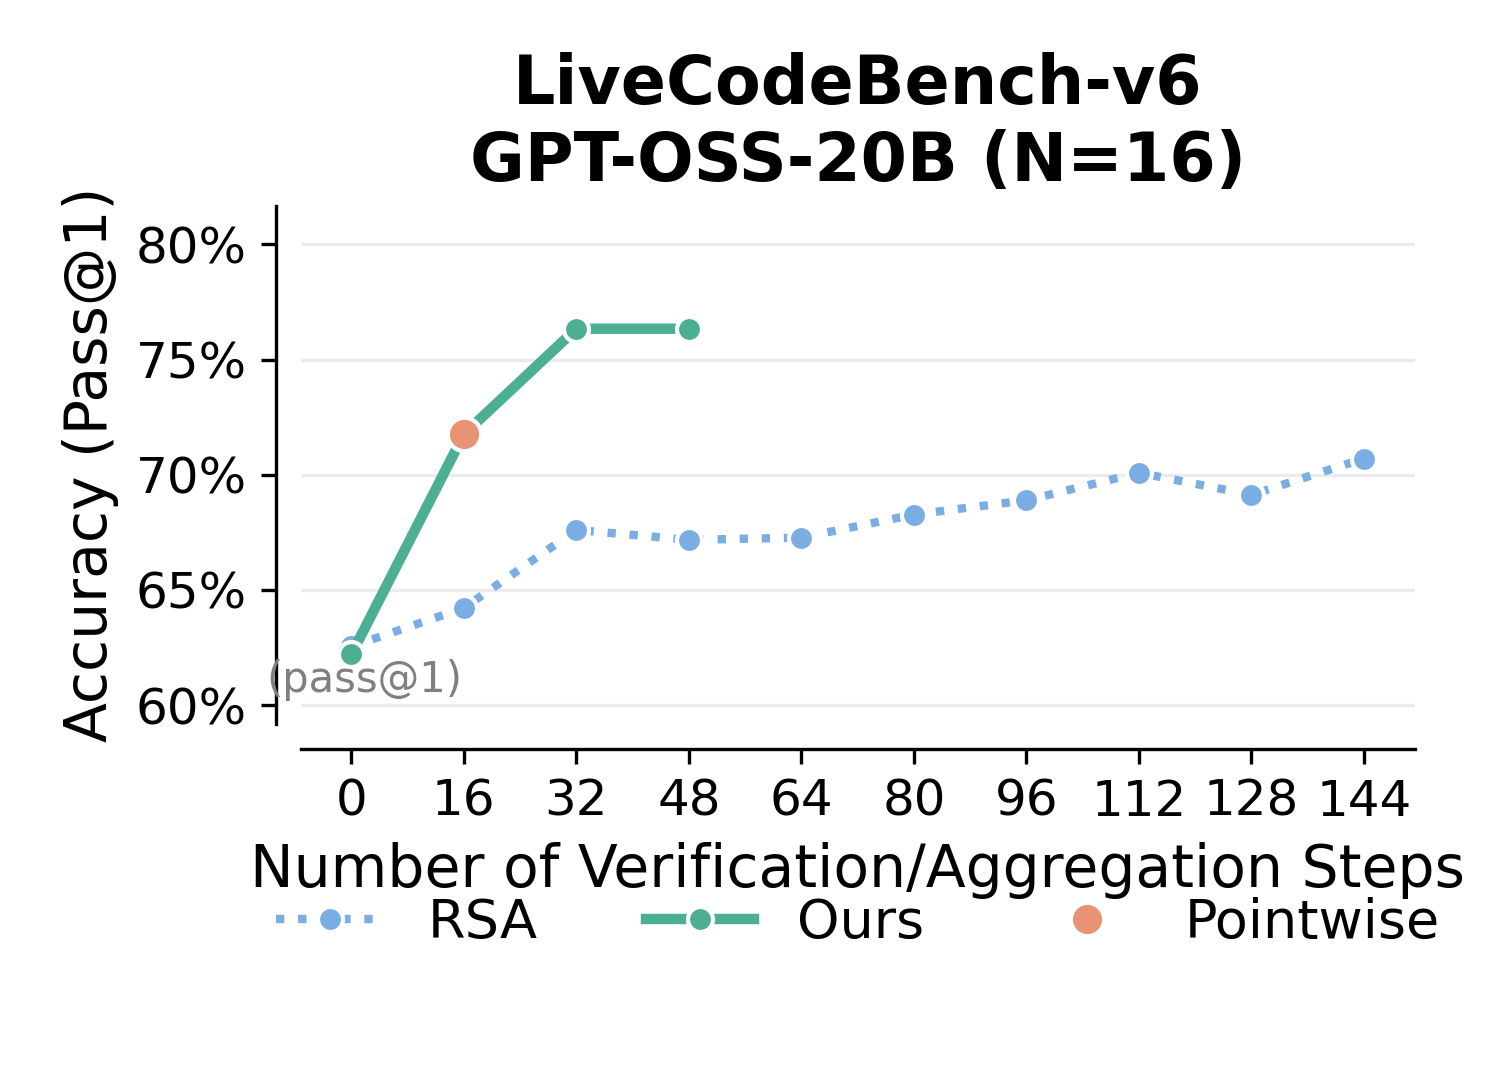
\includegraphics[width=0.35\textwidth]{images_verif/LiveCodeBench-v6_gpt-oss-20b_N16_LLMCalls_Comparison.png}
  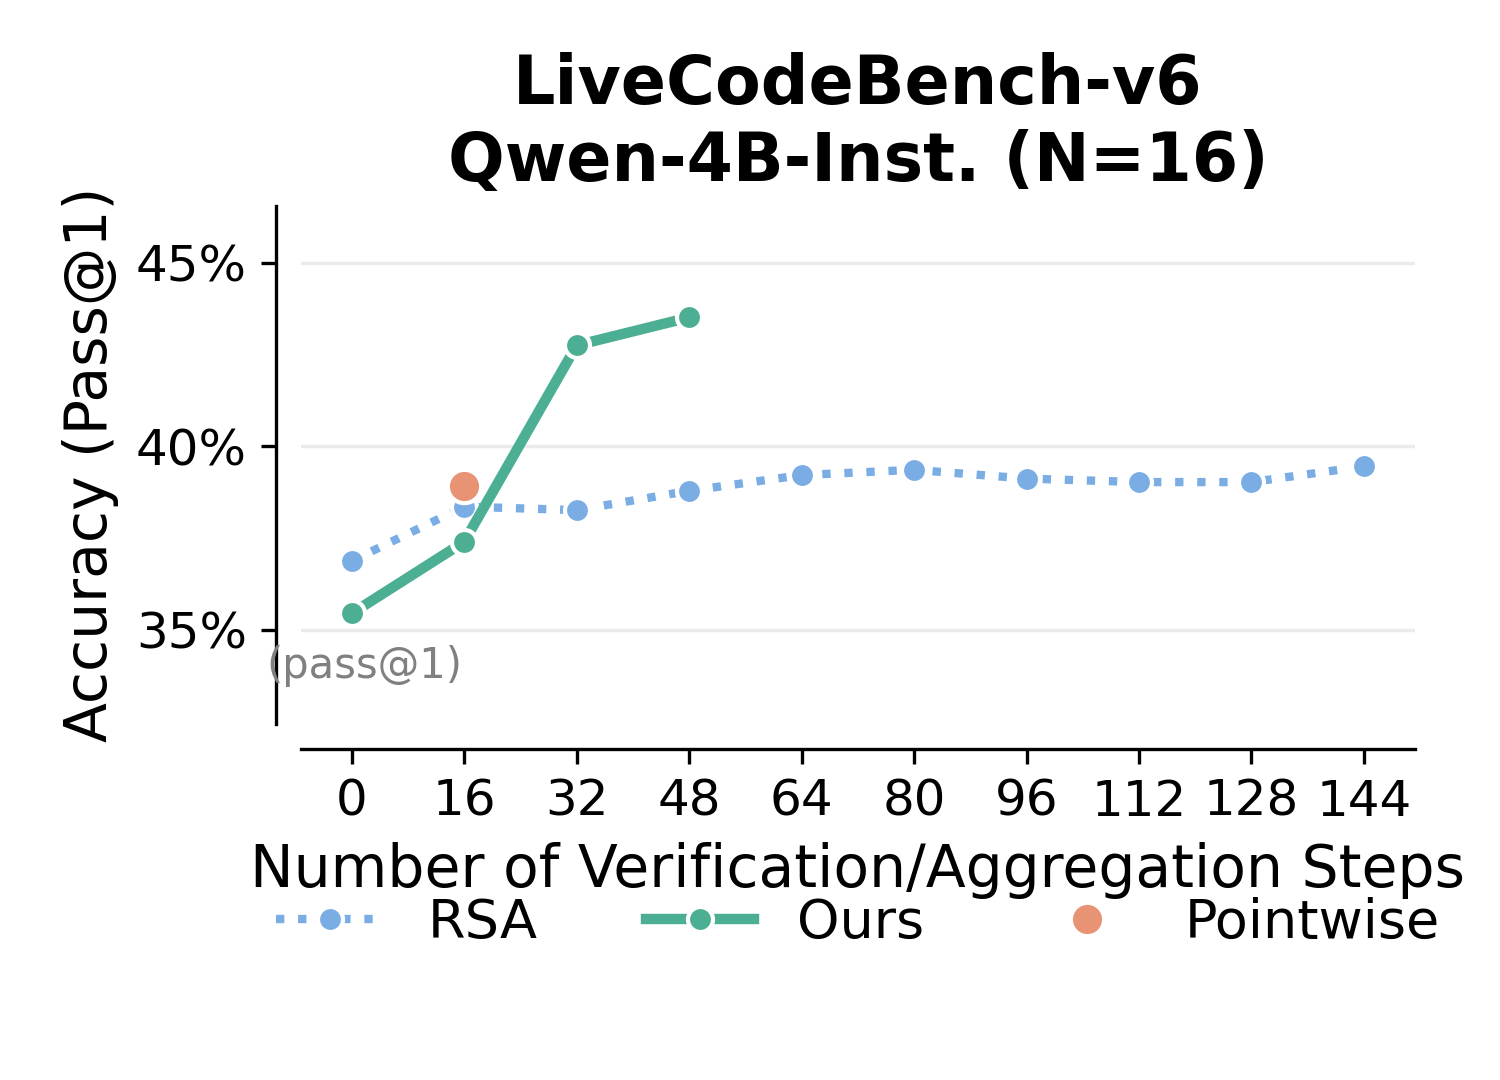
\includegraphics[width=0.35\textwidth]{images_verif/LiveCodeBench-v6_Qwen3-4B-Instruct-2507_N16_LLMCalls_Comparison.png}

  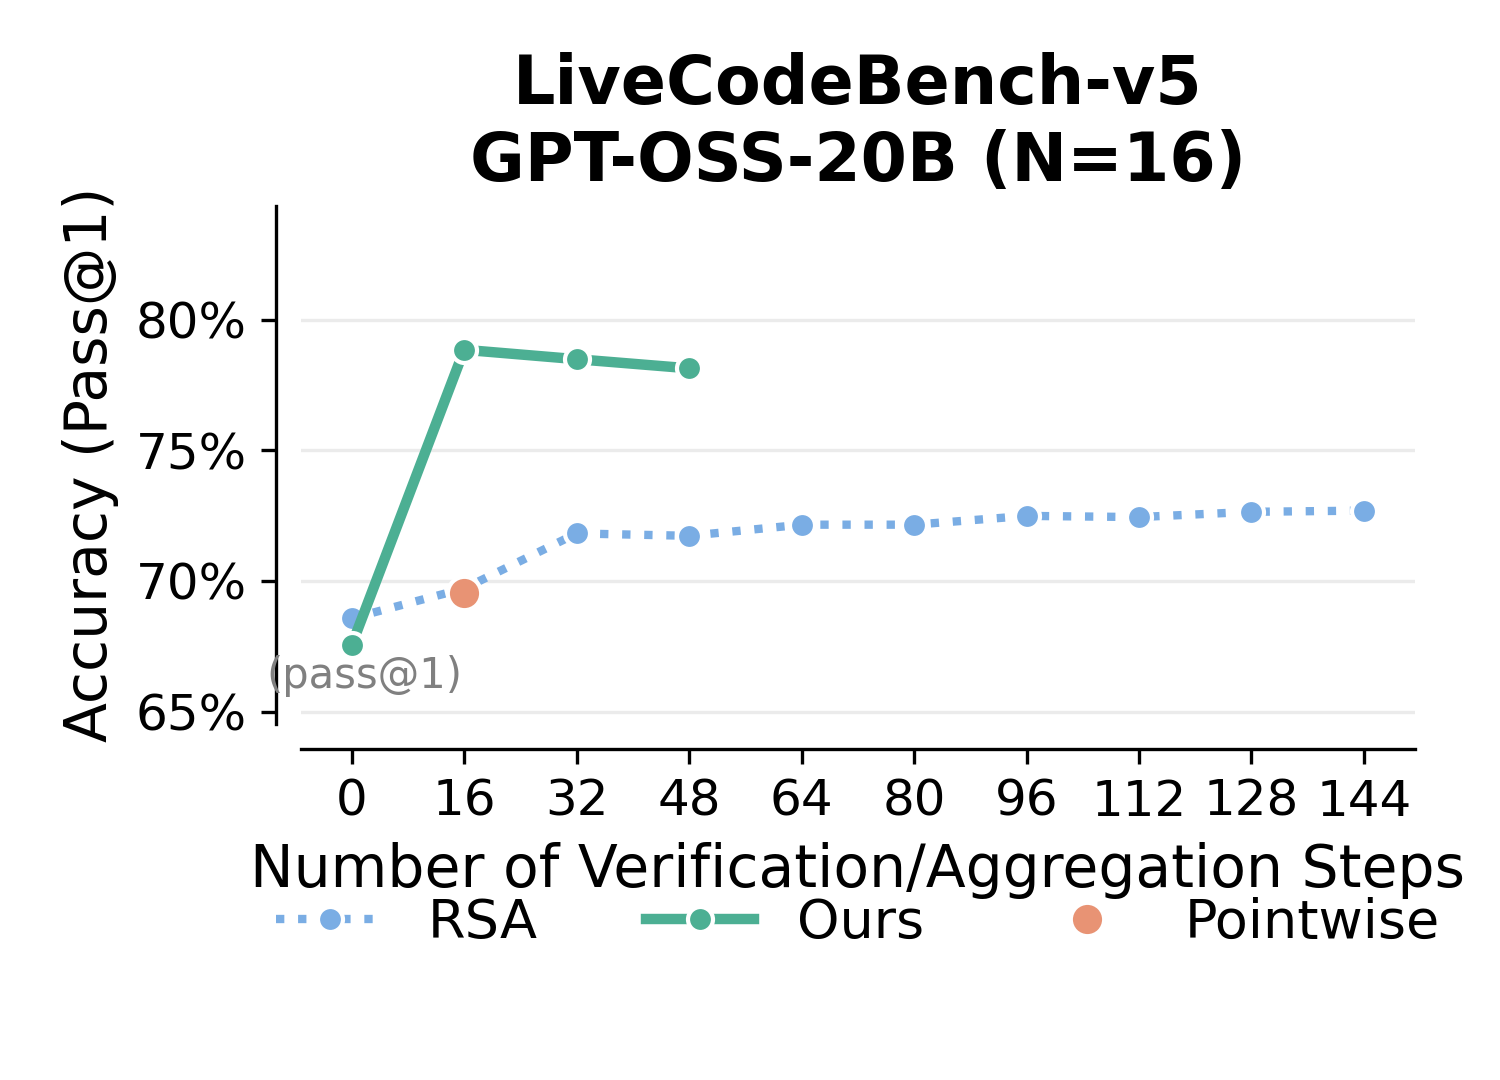
\includegraphics[width=0.35\textwidth]{images_verif/LiveCodeBench-v5_gpt-oss-20b_N16_LLMCalls_Comparison.png}
  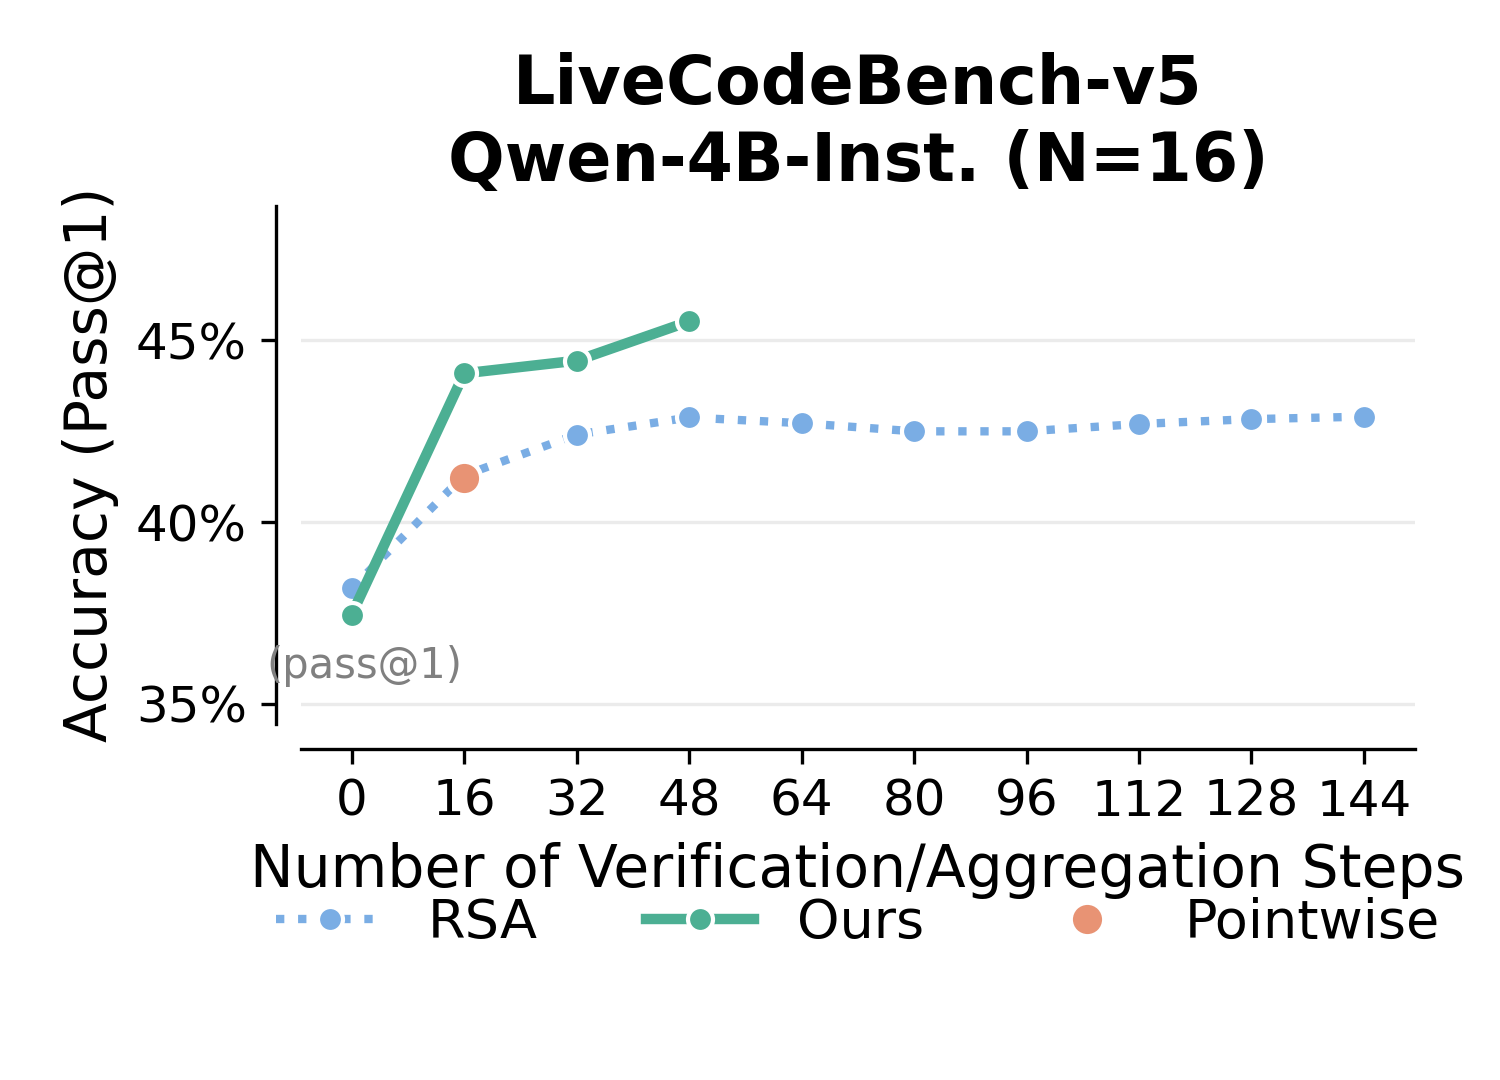
\includegraphics[width=0.35\textwidth]{images_verif/LiveCodeBench-v5_Qwen3-4B-Instruct-2507_N16_LLMCalls_Comparison.png}

  \caption{\textbf{Comparing Pairwise Verification with RSA.} Top row: LiveCodeBench-v6. Bottom row: LiveCodeBench-v5. Columns (left$\rightarrow$right): gpt-oss-20b, Qwen3-4B-Instruct-2507. \textbf{Here number of generations by the base model is 16}, followed by verification (pointwise, pairwise) or aggregation (RSA).}
  \label{fig:appendix_lcb_all_models_16}
\end{figure}

\begin{figure}[H]
  \centering
  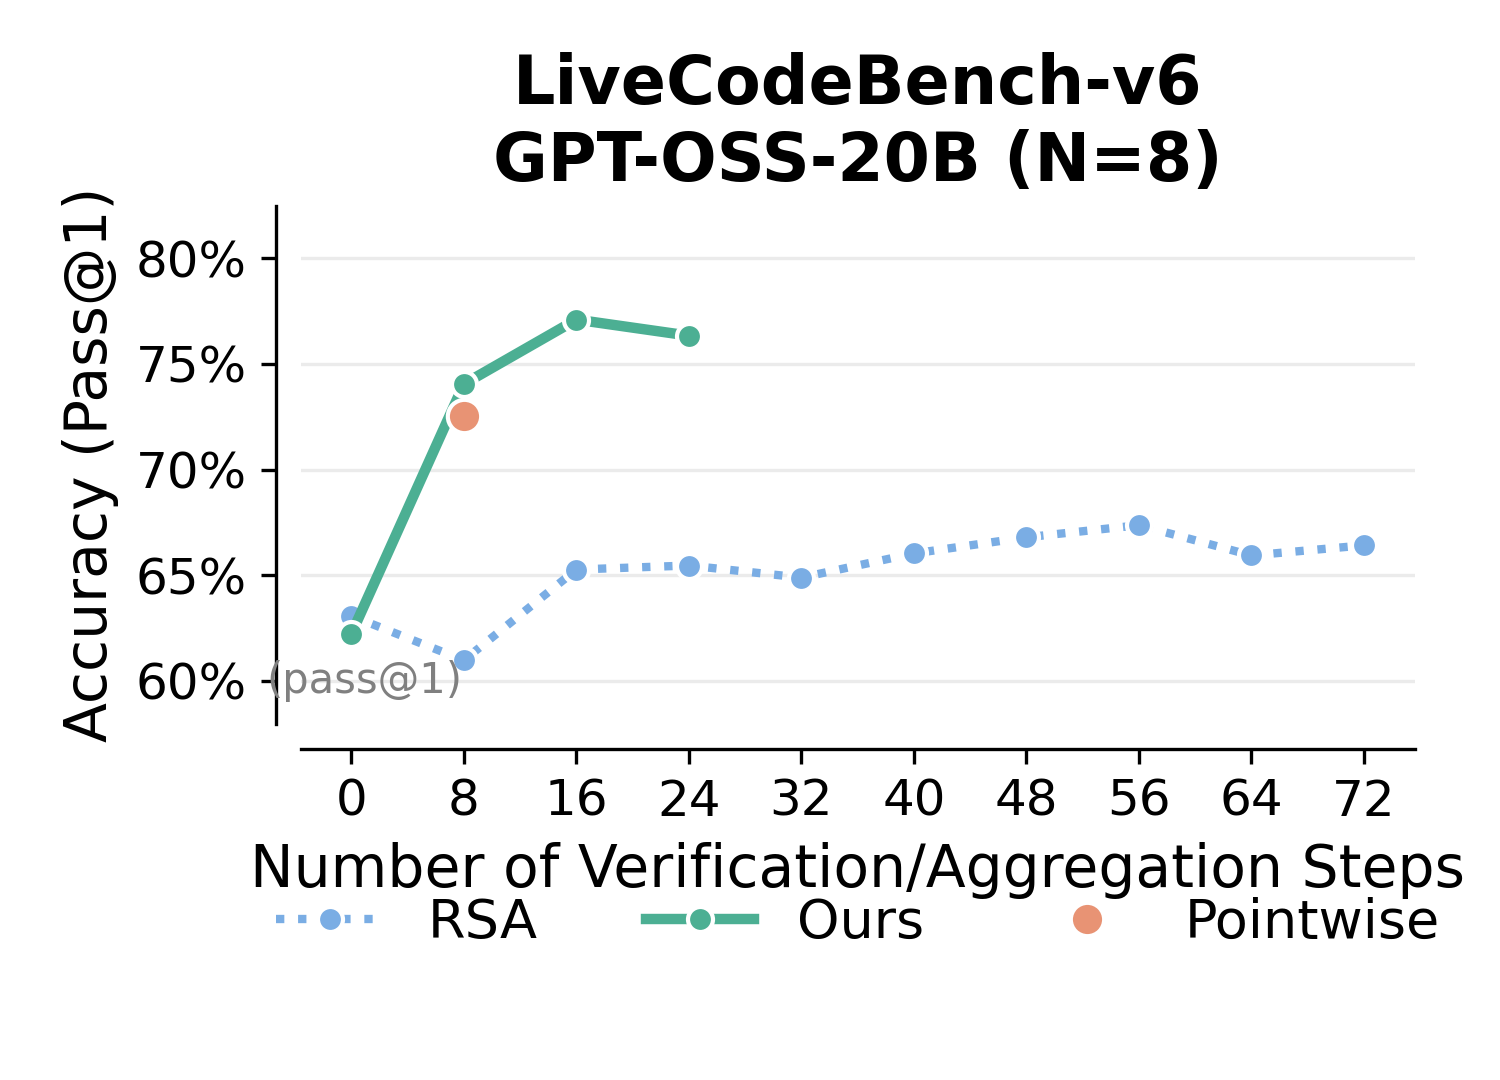
\includegraphics[width=0.35\textwidth]{images_verif/LiveCodeBench-v6_gpt-oss-20b_N8_LLMCalls_Comparison.png}
  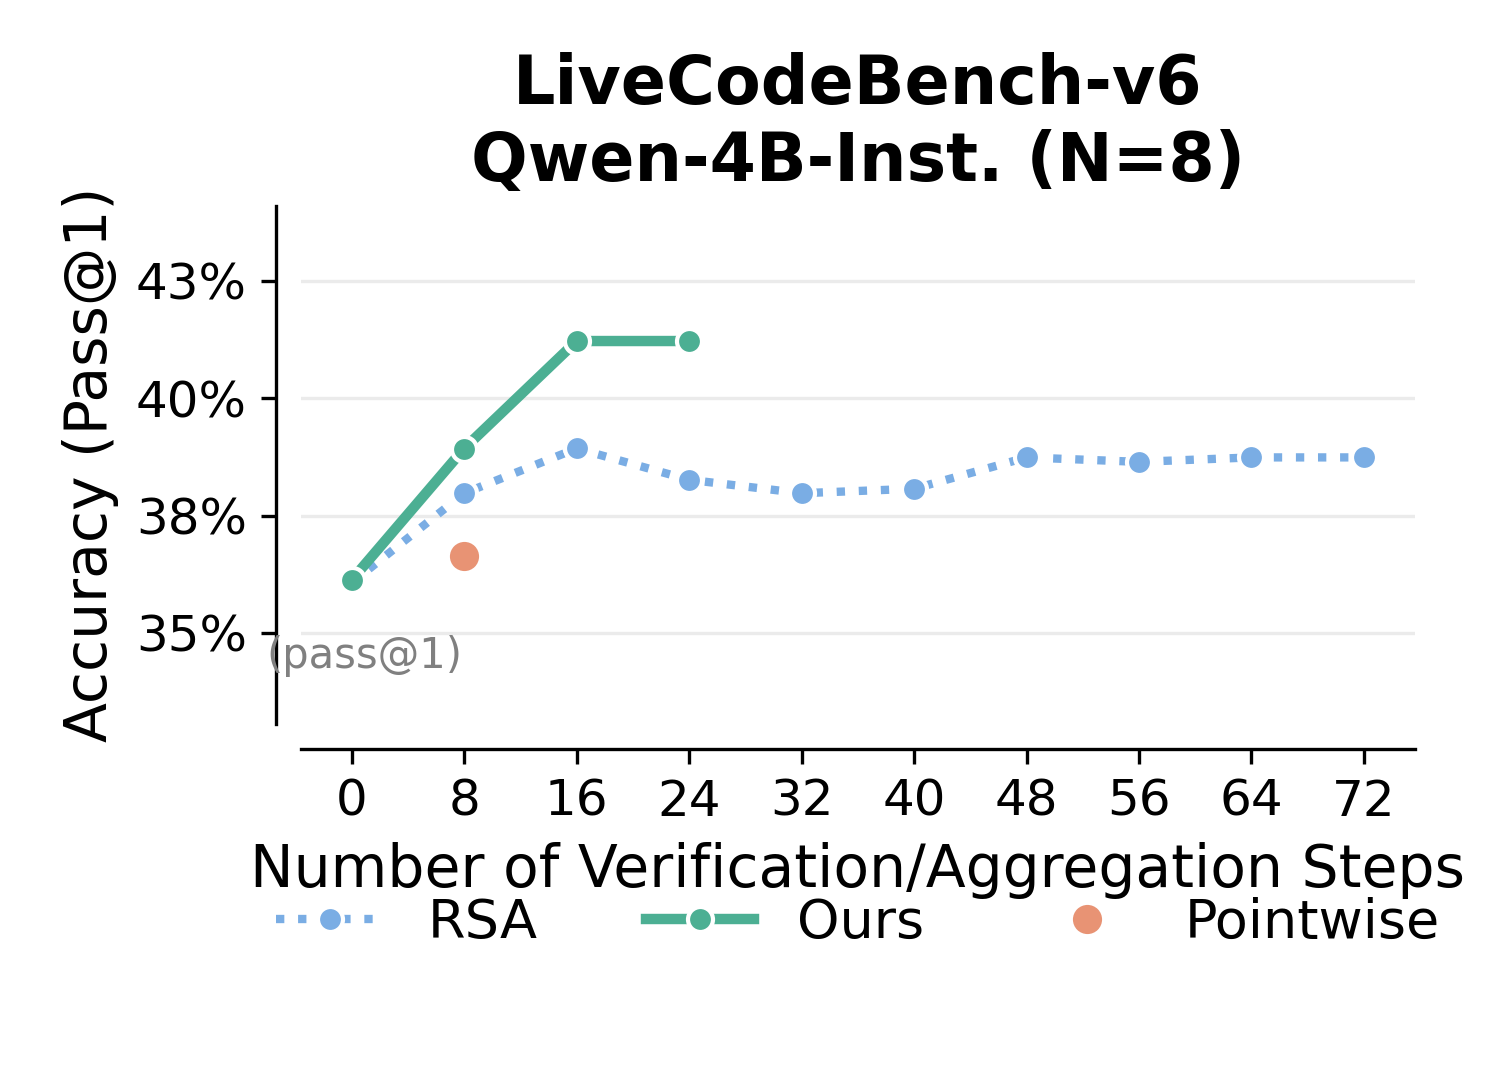
\includegraphics[width=0.35\textwidth]{images_verif/LiveCodeBench-v6_Qwen3-4B-Instruct-2507_N8_LLMCalls_Comparison.png}

  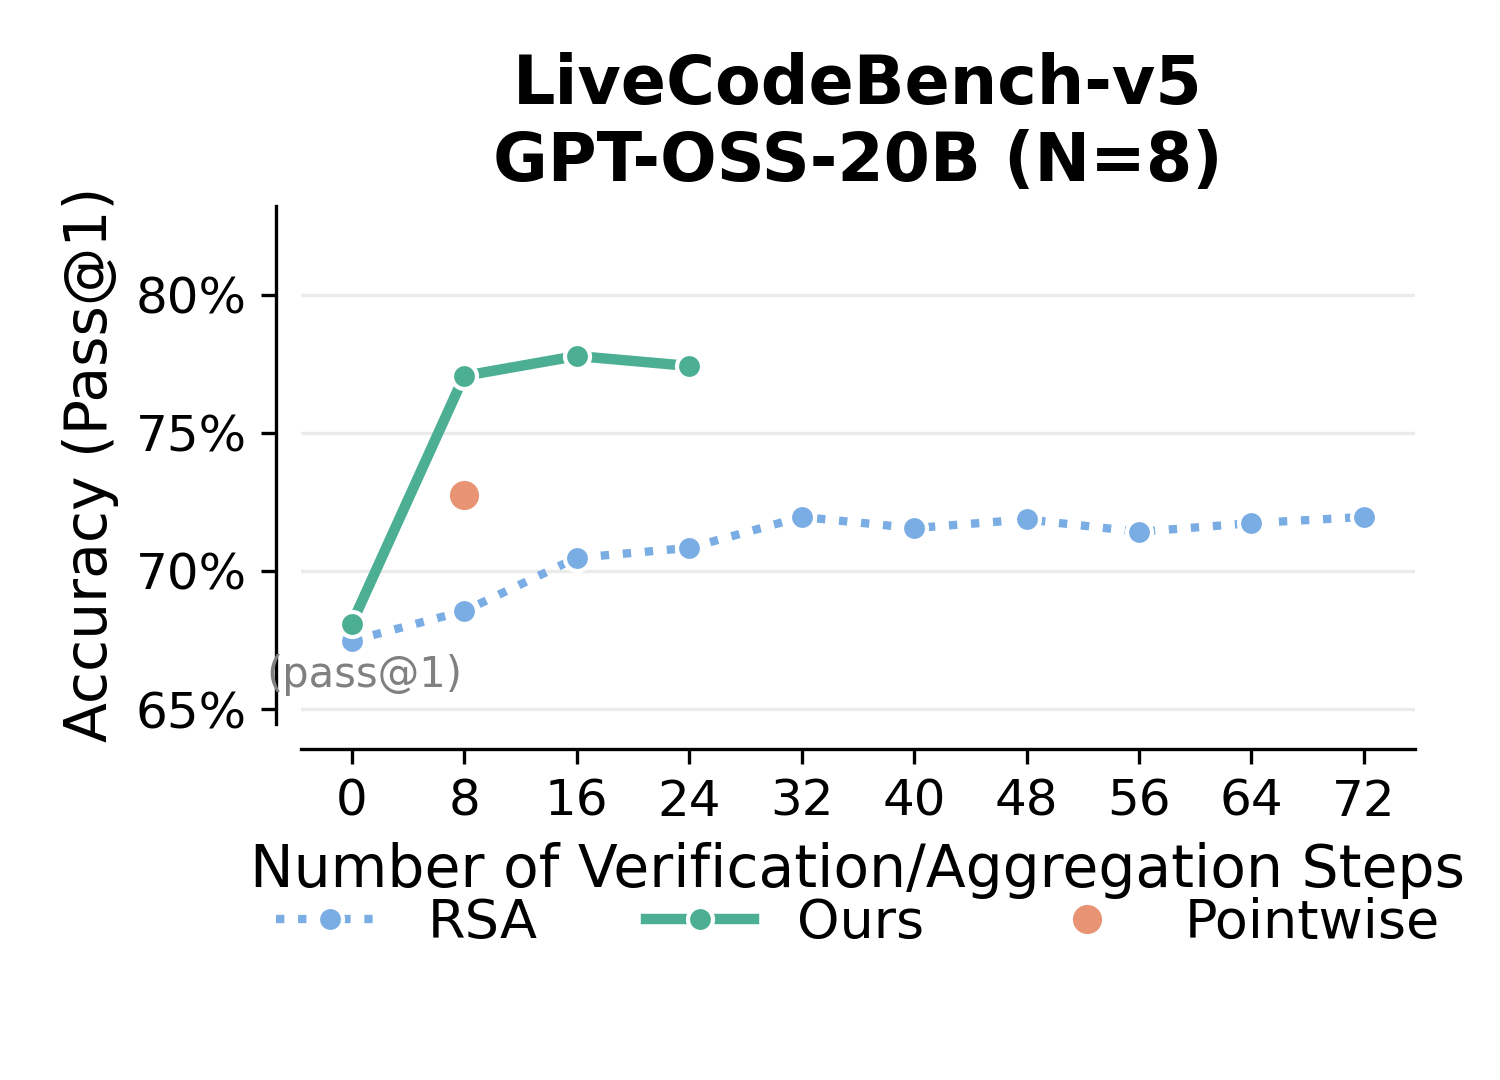
\includegraphics[width=0.35\textwidth]{images_verif/LiveCodeBench-v5_gpt-oss-20b_N8_LLMCalls_Comparison.png}
  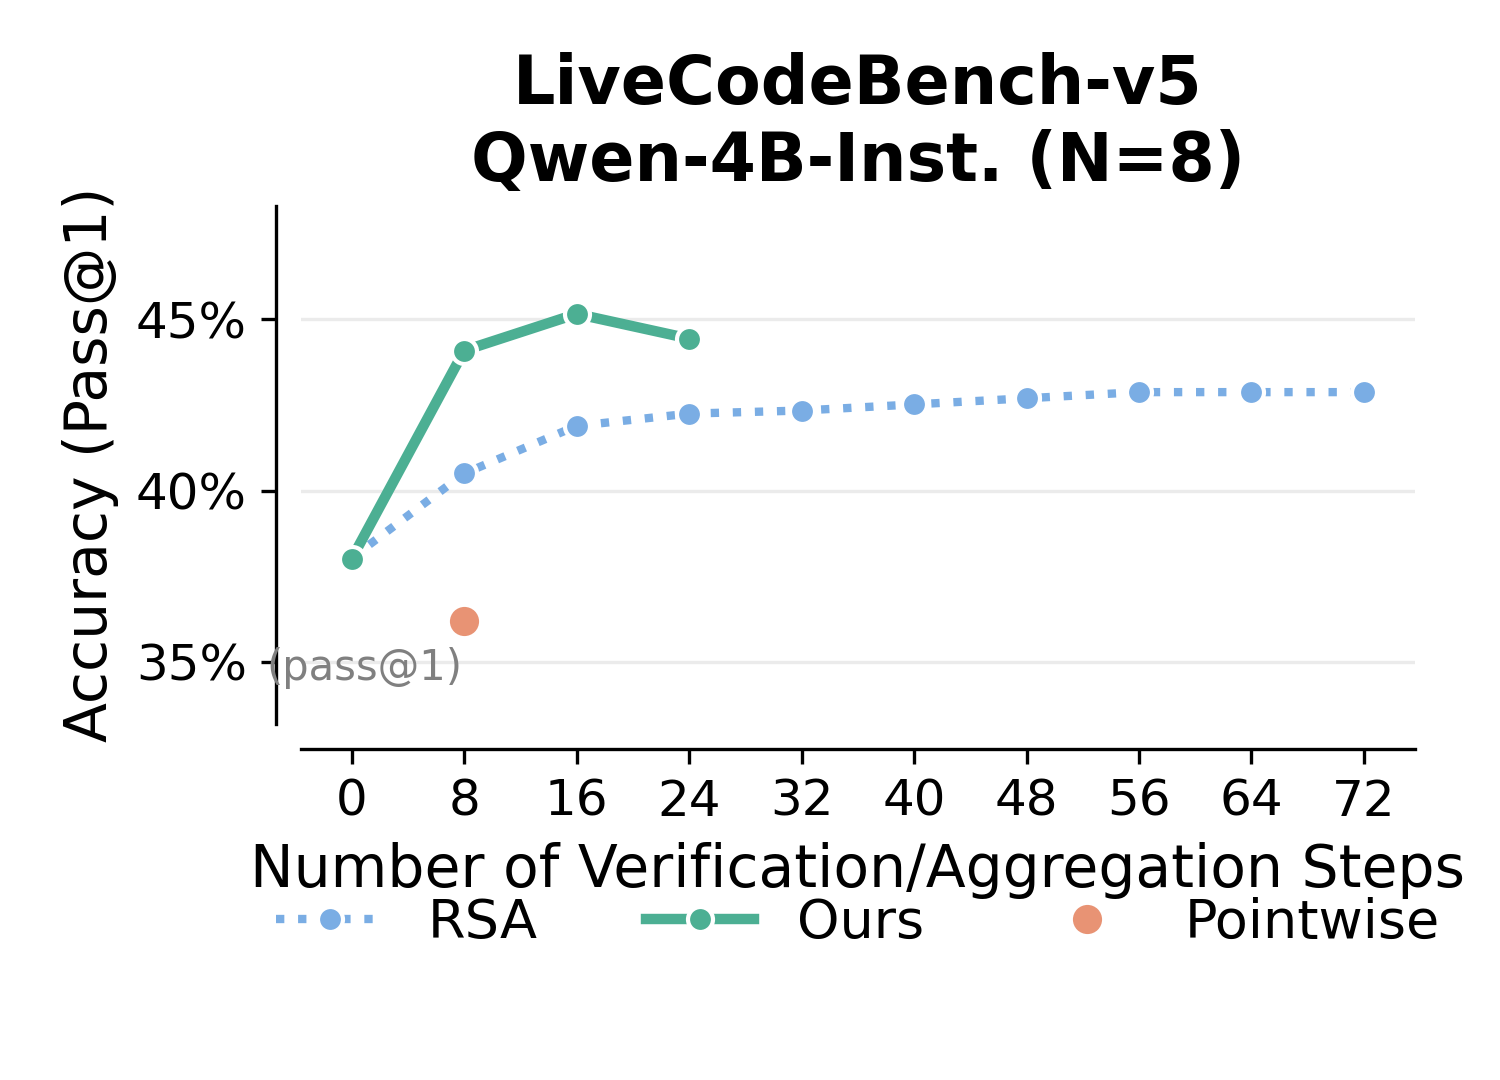
\includegraphics[width=0.35\textwidth]{images_verif/LiveCodeBench-v5_Qwen3-4B-Instruct-2507_N8_LLMCalls_Comparison.png}

  \caption{\textbf{Comparing Pairwise Verification with RSA.} Top row: LiveCodeBench-v6. Bottom row: LiveCodeBench-v5. Columns (left$\rightarrow$right): gpt-oss-20b, Qwen3-4B-Instruct-2507. \textbf{Here number of generations by the base model is 8}, followed by verification (pointwise, pairwise) or aggregation (RSA).}
  \label{fig:appendix_lcb_all_models_8}
\end{figure}


\begin{figure}[htbp]
  \centering
  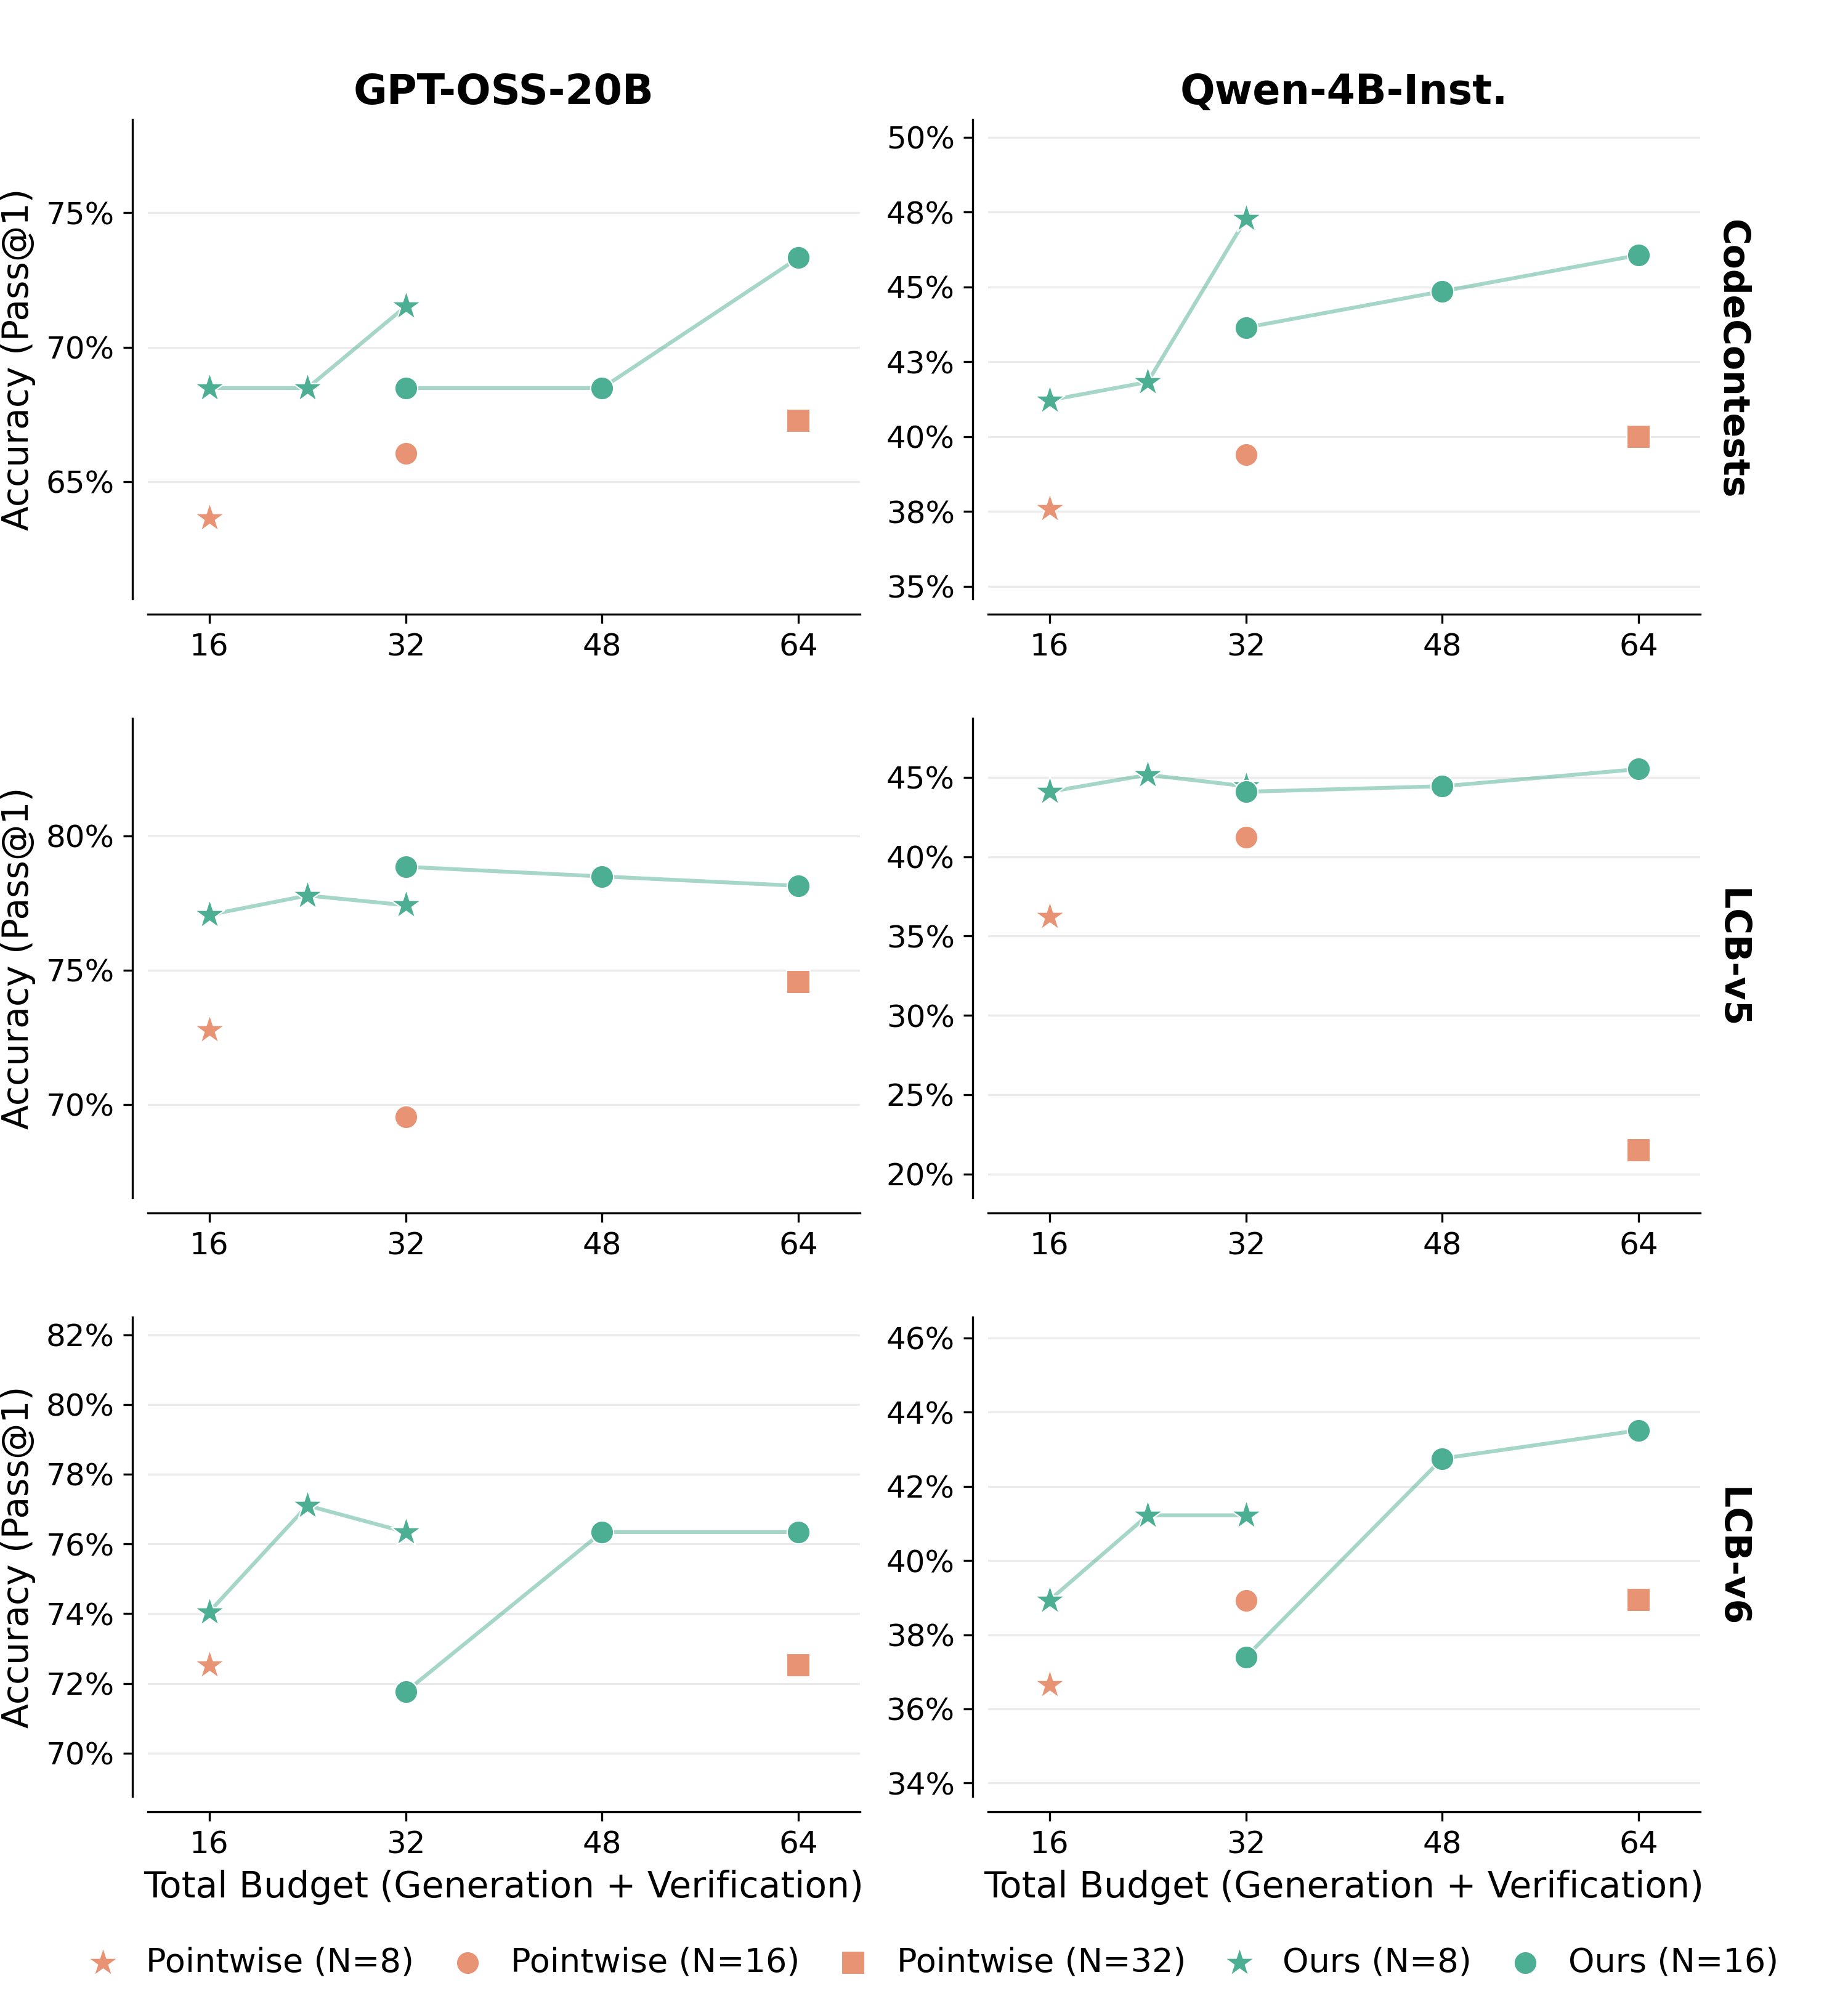
\includegraphics[width=0.85\textwidth]{images_verif/budget_vs_accuracy_per_benchmark.png}
  \caption{\textbf{Budget vs accuracy per benchmark.} Accuracy vs. total budget (generation + verification calls) for CodeContests (top row), LiveCodeBench-v5 (middle row), and LiveCodeBench-v6 (bottom row). Left column: GPT-OSS-20B. Right column: Qwen3-4B-Inst. Stars denote $N=8$ base generations, circles denote $N=16$, squares denote $N=32$ (pointwise only).}
  \label{fig:appendix_budget_per_benchmark}
\end{figure}


\clearpage
\section{Detailed Algorithm}
\label{sec:appendix_algo}

This section provides the full specification of the helper procedures used in
Algorithm~\ref{alg:ugpr}. The main paper presents a high-level view for clarity;
here we give the exact update rules and pairing strategies required for
reproducibility.


\paragraph{State.}
We maintain a state
$\mathcal{T} = (\{\mu_i\}_{i=1}^N, \{d_i\}_{i=1}^N, \mathcal{H})$,
where $\mu_i$ is the current estimated quality score of solution $s_i$,
$d_i$ is the number of distinct opponents it has been compared against,
and $\mathcal{H} \subset [N]\times[N]$ records previously compared pairs.

\paragraph{CoveragePairs.}
Ensures minimum degree while anchoring comparisons to similar-quality peers.
\begin{algorithm}[h]
\caption{\textsc{CoveragePairs}$(\mathcal{T}, d_{\min})$}
\label{alg:coveragepairs}
\begin{algorithmic}[1]
\Require State $\mathcal{T}=(\{\mu_i\},\{d_i\},\mathcal{H})$, minimum degree $d_{\min}$
\Ensure Disjoint pair set $\mathcal{P}$

\State $\mathcal{P}\gets\emptyset$, \ $\mathcal{U}\gets\emptyset$ \Comment{used indices}
\State $\mathcal{L}\gets\{i : d_i < d_{\min}\}$; sort $\mathcal{L}$ by increasing $d_i$

\For{each $i\in\mathcal{L}$}
    \If{$i\in\mathcal{U}$} \State \textbf{continue} \EndIf
    \State $\mathcal{C}\gets\{j\neq i : j\notin\mathcal{U},\ (i,j)\notin\mathcal{H}\}$
    \If{$\mathcal{C}=\emptyset$} \State \textbf{continue} \EndIf
    \State $j \gets \arg\min_{j\in\mathcal{C}} |\mu_i-\mu_j|$
    \State $\mathcal{P}\gets\mathcal{P}\cup\{(i,j)\}$
    \State $\mathcal{U}\gets\mathcal{U}\cup\{i,j\}$
\EndFor

\State \Return $\mathcal{P}$
\end{algorithmic}
\end{algorithm}

\paragraph{UpdateStats.}
This is where the mathematical aggregation is implemented.
\begin{algorithm}[h]
\caption{\textsc{UpdateStats}$(\mathcal{T},\mathcal{O},\tau)$}
\label{alg:updatestats}
\begin{algorithmic}[1]
\Require State $\mathcal{T}=(\{\mu_i\},\{d_i\},\mathcal{H})$, outcomes $\mathcal{O}$, floor $\tau>0$
\Ensure Updated state $\mathcal{T}$

\For{each $(i,j,w,r_i,r_j)\in\mathcal{O}$}
    \State $v_{ij}\gets \mathbb{I}[w=\texttt{A}] + 0.5\cdot\mathbb{I}[w=\texttt{tie}]$
    \State $w_{ij}\gets \max\!\left(\frac{|r_i-r_j|}{9},\tau\right)$
    \State update $\mu_i,\mu_j$ using Eq.~(1)
    \If{$(i,j)\notin\mathcal{H}$}
        \State $d_i\gets d_i+1$;\quad $d_j\gets d_j+1$
        \State $\mathcal{H}\gets\mathcal{H}\cup\{(i,j),(j,i)\}$
    \EndIf
\EndFor
\end{algorithmic}
\end{algorithm}
Note. In practice, the update of $\mu_i$ is implemented incrementally using sufficient statistics, but Eq.~(1) fully specifies the aggregation semantics.

\paragraph{SwissPairs.}
Allocates remaining budget to the most informative near-ties.
\begin{algorithm}[h]
\caption{\textsc{SwissPairs}$(\pi,\mathcal{T},h)$}
\label{alg:swisspairs}
\begin{algorithmic}[1]
\Require Ranking $\pi$, state $\mathcal{T}=(\{\mu_i\},\{d_i\},\mathcal{H})$, window size $h$
\Ensure Disjoint pair set $\mathcal{P}$

\State $\mathcal{P}\gets\emptyset$, \ $\mathcal{U}\gets\emptyset$
\For{$k=1$ \textbf{to} $N$}
    \State $i\gets\pi_k$
    \If{$i\in\mathcal{U}$} \State \textbf{continue} \EndIf
    \State $\mathcal{C}\gets\emptyset$
    \For{$t=k+1$ \textbf{to} $\min(k+h,N)$}
        \State $j\gets\pi_t$
        \If{$j\in\mathcal{U}$} \State \textbf{continue} \EndIf
        \State add $(|\mu_i-\mu_j|,\mathbb{I}[(i,j)\in\mathcal{H}],j)$ to $\mathcal{C}$
    \EndFor
    \If{$\mathcal{C}\neq\emptyset$}
        \State choose $j$ with lexicographically minimal key in $\mathcal{C}$
        \State $\mathcal{P}\gets\mathcal{P}\cup\{(i,j)\}$
        \State $\mathcal{U}\gets\mathcal{U}\cup\{i,j\}$
    \EndIf
\EndFor

\State \Return $\mathcal{P}$
\end{algorithmic}
\end{algorithm}


The above procedures jointly ensure (i) early stabilization of the comparison
topology via minimum-degree coverage and (ii) efficient use of remaining budget
through uncertainty-focused Swiss refinement, enabling accurate ranking with
$O(N)$–scale pairwise verification.


\begin{figure}[htbp]
  \centering
  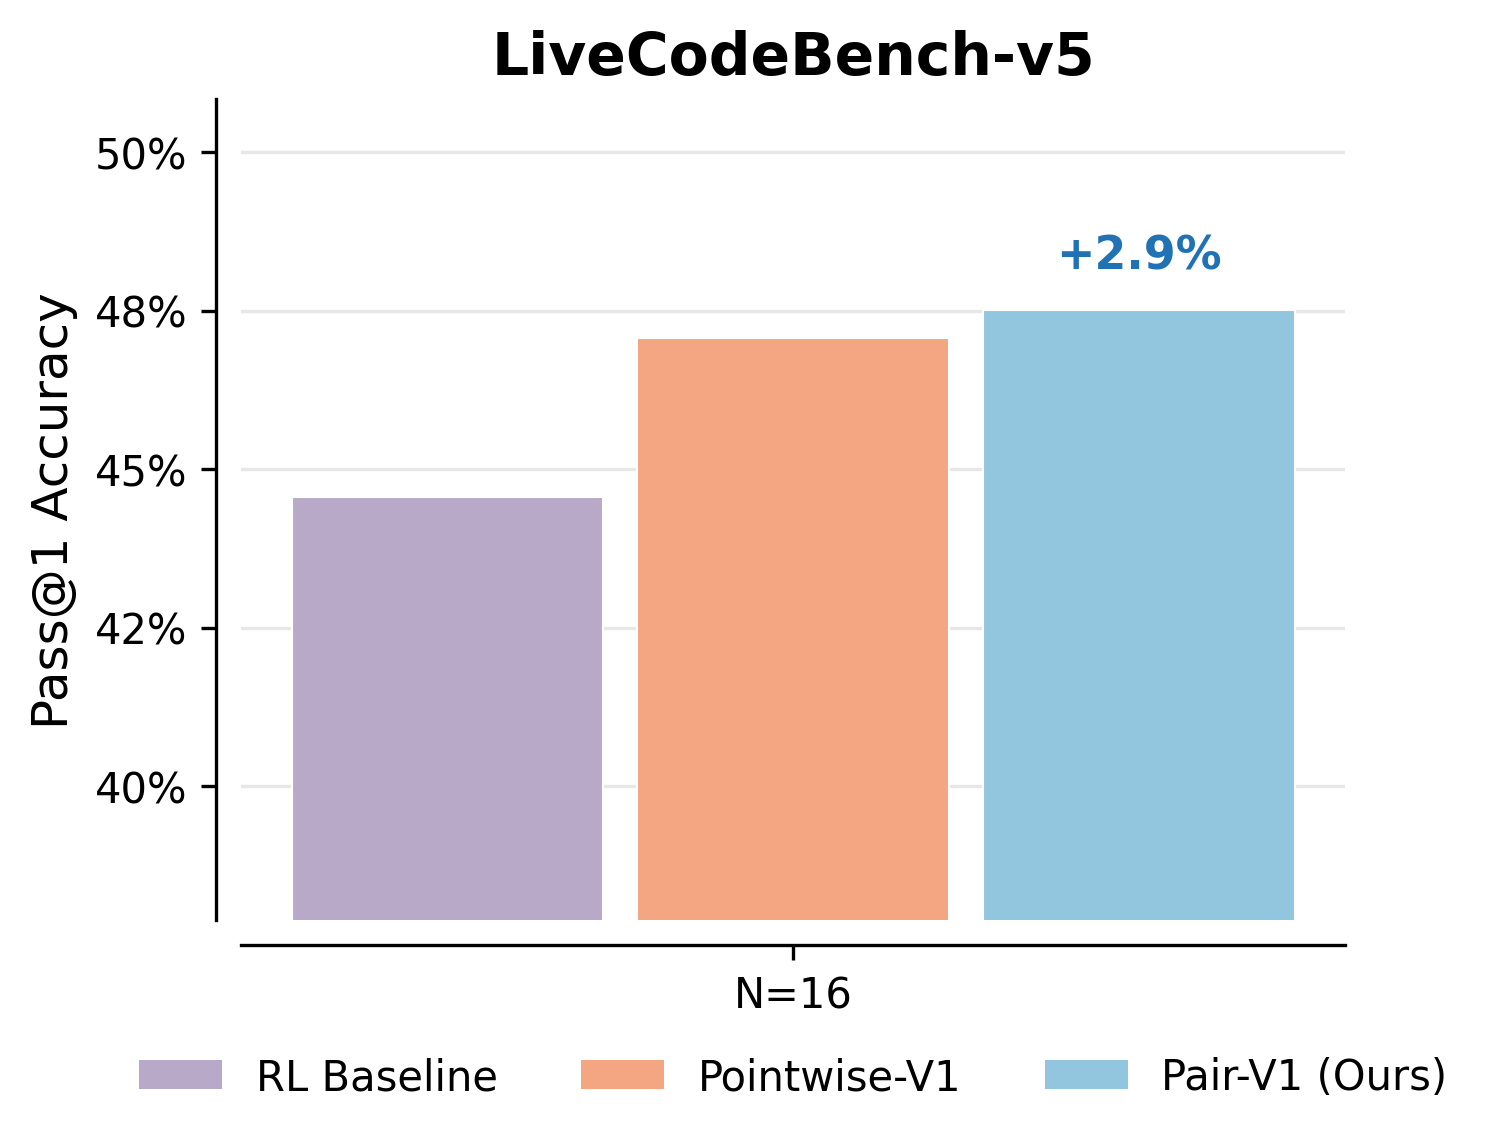
\includegraphics[width=0.32\textwidth]{images_verif/LiveCodeBench_v5_TrainedModels_Pass1_N16.png}\hfill
  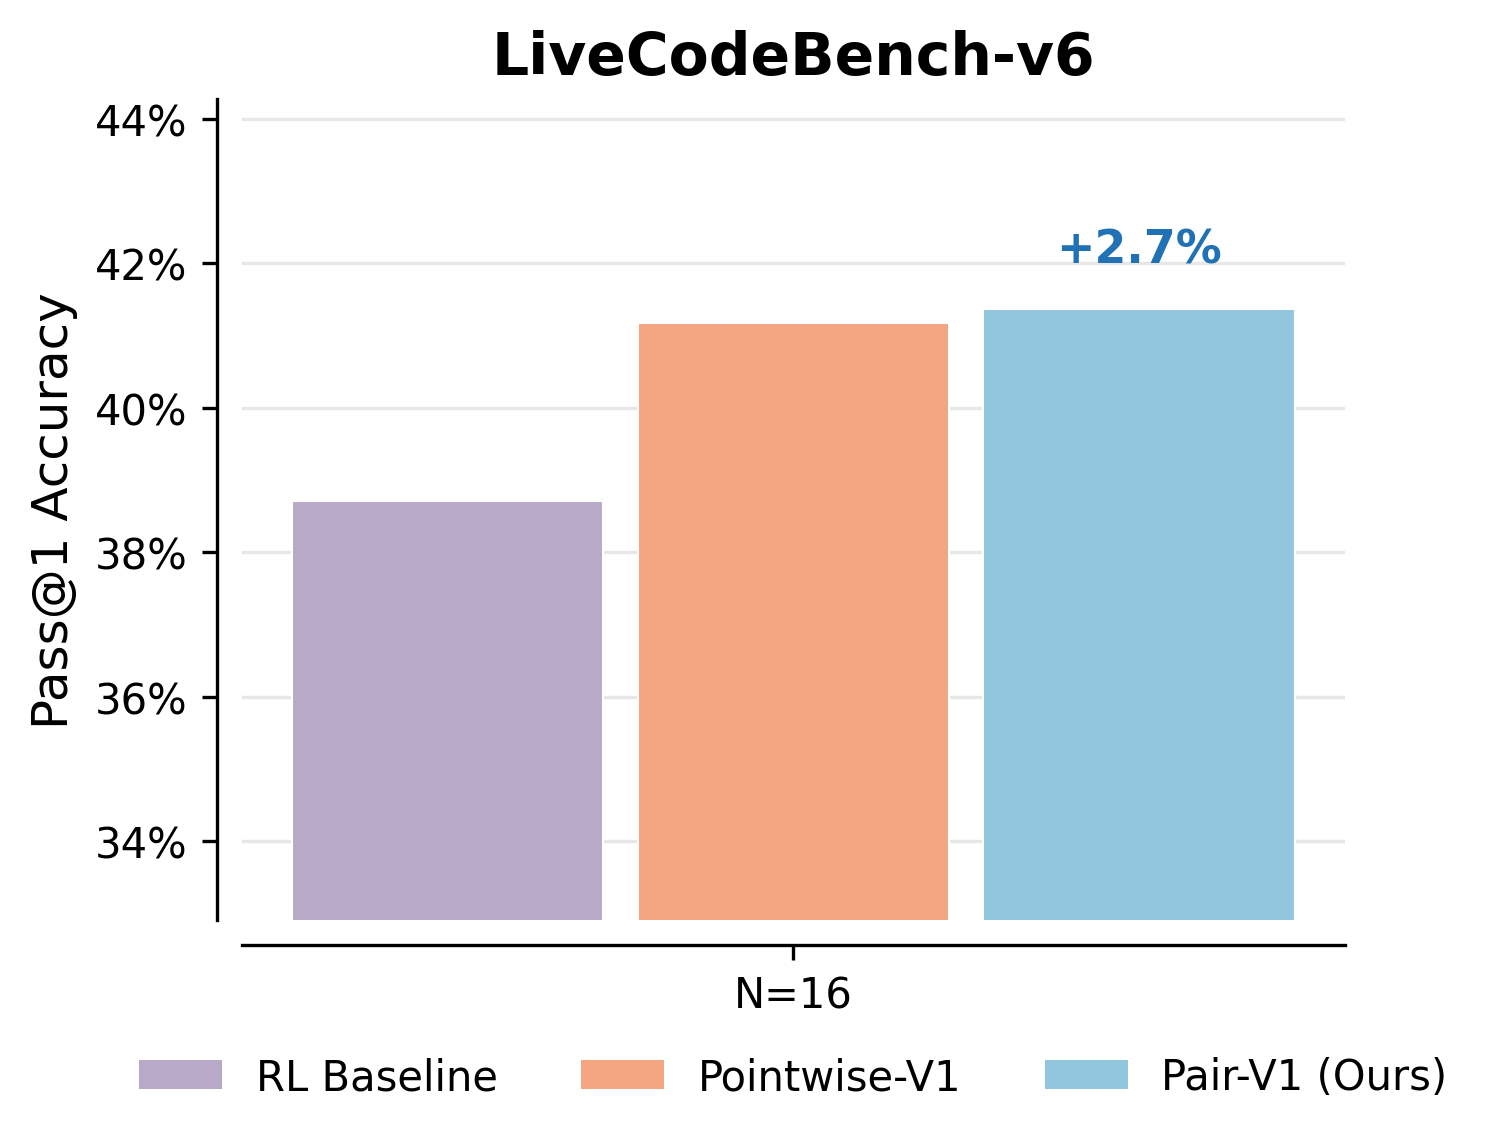
\includegraphics[width=0.32\textwidth]{images_verif/LiveCodeBench_v6_TrainedModels_Pass1_N16.png}\hfill
  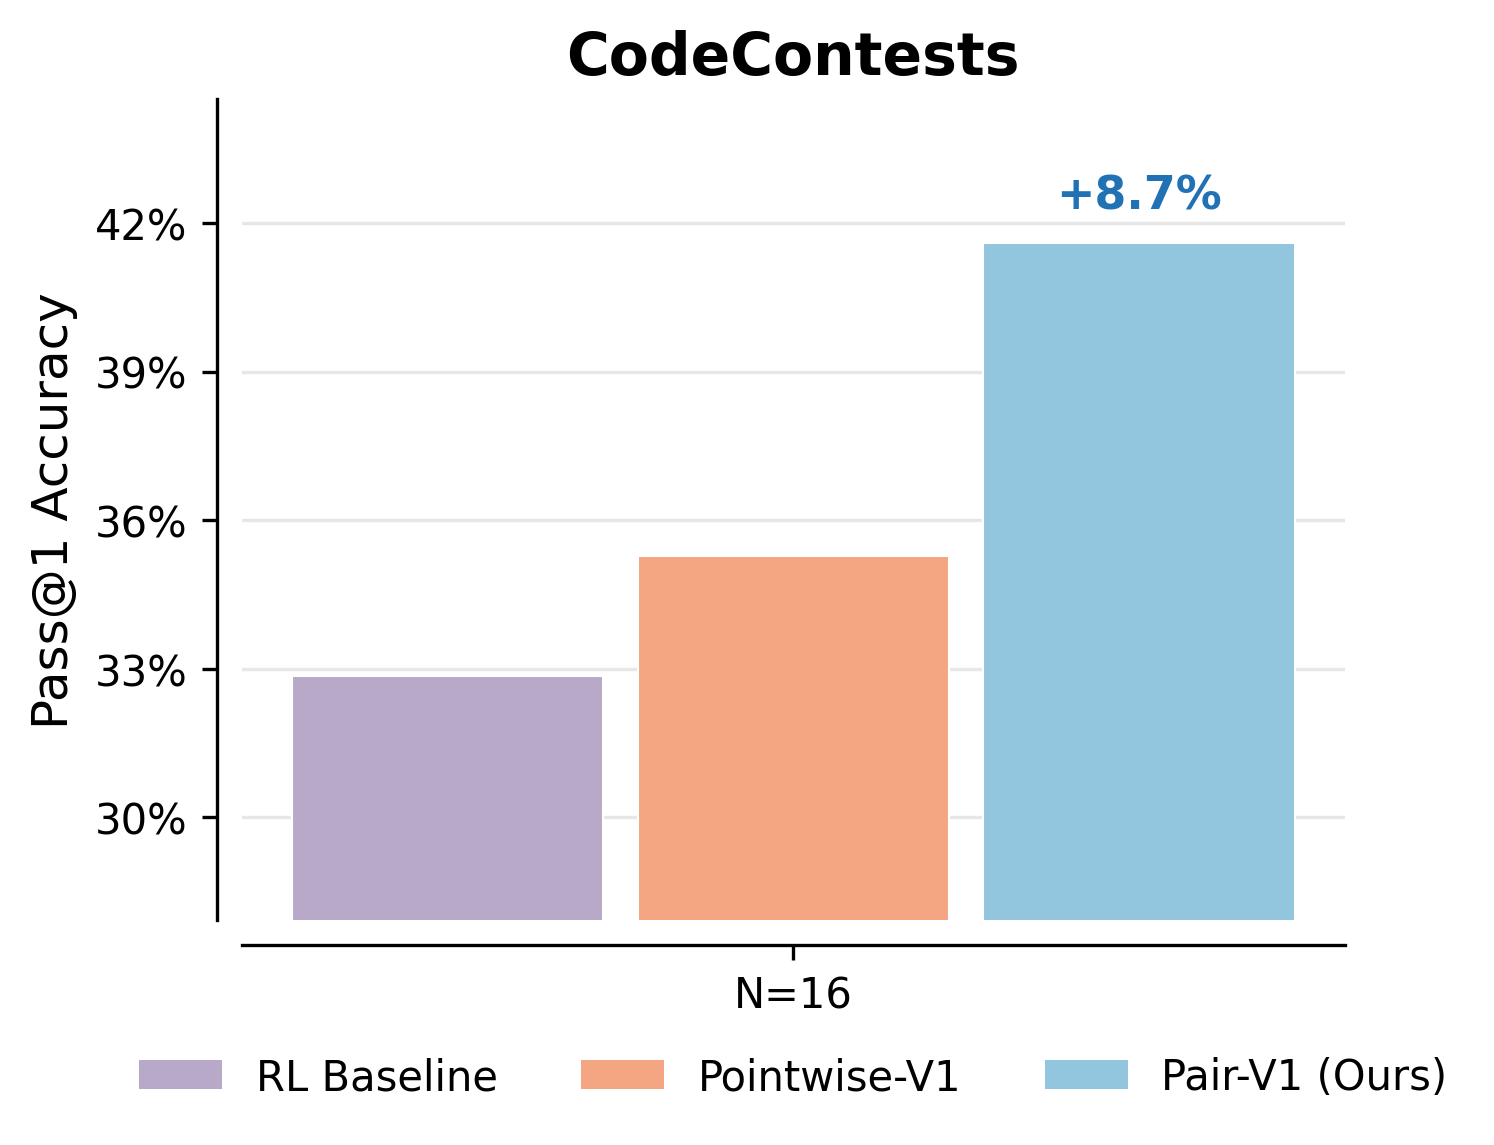
\includegraphics[width=0.32\textwidth]{images_verif/CodeContests_TrainedModels_Pass1_N16.png}
  \caption{\textbf{\method{}-PairRL vs RL baseline across benchmarks (N=16).}
  Left: LiveCodeBench-v5. Middle: LiveCodeBench-v6. Right: CodeContests. Co-training with pairwise verification consistently improves Pass@1 accuracy across all benchmarks.}
  \label{fig:pairv1_vs_rl_per_benchmark}
\end{figure}


\clearpage
\section{Generation Prompts}
\label{sec:generation_prompts}


\subsection{Code Generation}

\begin{tcolorbox}[
    colback=promptbg,
    colframe=promptborder,
    title={\textbf{Code Generation Prompt}},
    coltitle=white,
    fonttitle=\small\bfseries,
    breakable,
    enhanced
]
\small
\ttfamily
\textbf{**Problem**}\\
\{problem\}\\[0.75em]

Think and reason step by step before coding the final solution for the problem above.
Put your reasoning and any draft coding solutions between <thinking> ... </thinking> tags.
After the reasoning (i.e. after the </thinking> tag), use the format provided in the problem above
(code-block with backticks) to format your final code solution. Do not include any thinking within the code block.\\[0.75em]

\#\#\# Answer:
\end{tcolorbox}

Note that "Do not include any thinking within the code-block." is added to the prompt, since in the absence of it, training the model
(Qwen3-4B-Instruct-2507) leads to it generating large amounts of comments within the code block, effectively leading to truncation of the response (due to reaching max length) and hence, 0 rewards and training collapse.

\subsection{Math Solution Generation}

\begin{tcolorbox}[
    colback=promptbg,
    colframe=promptborder,
    title={\textbf{Math Solution Generation Prompt}},
    coltitle=white,
    fonttitle=\small\bfseries,
    breakable,
    enhanced
]
\small
\ttfamily
\{problem\}. Let's think step by step and output the final answer within \textbackslash boxed\{\}.
\end{tcolorbox}


\clearpage
\section{Verification Prompts}
\label{sec:appendix_prompts}

This section provides the exact prompts used for pointwise and pairwise self-verification in our experiments. Both verification methods use a 1--10 rating scale for fair comparison.

\subsection{Pointwise Verification Prompts}

\subsubsection{Code Generation}

\begin{tcolorbox}[
    colback=promptbg,
    colframe=promptborder,
    title={\textbf{Pointwise Code Verification Prompt}},
    coltitle=white,
    fonttitle=\small\bfseries,
    breakable,
    enhanced
]
\small
\ttfamily
You are an expert code reviewer. Rate the correctness of a solution to a programming problem.\\[0.5em]
\textbf{**Evaluation Guidelines:**}\\
- Analyze the problem's requirements and constraints.\\
- Mentally trace the solution with test cases (including edge cases) to verify correctness.\\
- Give a higher score if the solution is robust and fault-tolerant.\\[0.5em]
\textbf{**Problem**}\\
\{problem\}\\[0.5em]
\textbf{**Solution**}\\
\{code\}\\[0.5em]
\textbf{**Output Format:**}\\
First, provide your step-by-step reasoning. Then, on a new line, provide your final rating using the EXACT tags below. Add no other text after the tags.\\
<rating>INTEGER\_1\_TO\_10</rating>\\[0.5em]
\textbf{**Rating Rules:**}\\
- Rate correctness on a 1-10 scale (10 = correct \& robust, 5 = borderline, 1 = incorrect).\\
Please provide your analysis now.
\end{tcolorbox}

\subsubsection{Math Reasoning}

\begin{tcolorbox}[
    colback=promptbg,
    colframe=promptborder,
    title={\textbf{Pointwise Math Verification Prompt}},
    coltitle=white,
    fonttitle=\small\bfseries,
    breakable,
    enhanced
]
\small
\ttfamily
You are an expert math contest grader. Rate the correctness of a submission based solely on the final answer.\\[0.5em]
\textbf{**Evaluation Guidelines:**}\\
- Extract the submission's final answer. Use any provided reasoning only to help you assess whether the stated final answer is trustworthy. Do not award credit for method quality or rigor.\\
- Carefully analyze the problem statement and the submission to assess whether the final answer is correct. Grade only the final answer.\\[0.5em]
\textbf{**Problem**}\\
\{problem\}\\[0.5em]
\textbf{**Solution**}\\
\{solution\}\\[0.5em]
\textbf{**Output Format:**}\\
First, provide your reasoning (what checks you performed). Then, on a new line, provide your final rating using the EXACT tag below. Add no other text after the tag.\\
<rating>INTEGER\_1\_TO\_10</rating>\\[0.5em]
\textbf{**Rating Rules:**}\\
- Rate correctness on a 1-10 scale (10 = certainly correct, 8 = very likely correct, 5 = uncertain/borderline, 3 = likely incorrect, 1 = certainly incorrect).\\
Please provide your analysis now.
\end{tcolorbox}

\subsection{Pairwise Verification Prompts}

\subsubsection{Code Generation}

\begin{tcolorbox}[
    colback=promptbg,
    colframe=promptborder,
    title={\textbf{Pairwise Code Verification Prompt}},
    coltitle=white,
    fonttitle=\small\bfseries,
    breakable,
    enhanced
]
\small
\ttfamily
You are an expert code reviewer. Compare two solutions to a programming problem and rate their correctness.\\[0.5em]
\textbf{**Evaluation Guidelines:**}\\
- Analyze the problem's requirements and constraints.\\
- Mentally trace each solution with test cases (including edge cases) to verify correctness.\\
- If both solutions appear correct, prefer the more robust and fault-tolerant one.\\[0.5em]
\textbf{**Problem**}\\
\{problem\}\\[0.5em]
\textbf{**Solution A**}\\
\{code\_A\}\\[0.5em]
\textbf{**Solution B**}\\
\{code\_B\}\\[0.5em]
\textbf{**Output Format:**}\\
First, provide your step-by-step reasoning. Then, on separate new lines, provide your final ratings using the EXACT tags below. Add no other text after the tags.\\
<rating\_A>INTEGER\_1\_TO\_10</rating\_A>\\
<rating\_B>INTEGER\_1\_TO\_10</rating\_B>\\[0.5em]
\textbf{**Rating Rules:**}\\
- Rate correctness on a 1-10 scale (10 = correct \& robust, 5 = borderline, 1 = incorrect).\\
- The higher rating wins. Equal ratings imply a tie.\\
Please provide your analysis now.
\end{tcolorbox}

\subsubsection{Math Reasoning}

\begin{tcolorbox}[
    colback=promptbg,
    colframe=promptborder,
    title={\textbf{Pairwise Math Verification Prompt}},
    coltitle=white,
    fonttitle=\small\bfseries,
    breakable,
    enhanced
]
\small
\ttfamily
You are an expert math contest grader. Compare two submissions and rate correctness based solely on the final answer.\\[0.5em]
\textbf{**Evaluation Guidelines:**}\\
- Extract each submission's final answer. Use any provided reasoning only to help you assess whether the stated final answer is trustworthy. Do not award credit for method quality or rigor.\\
- Carefully analyze the problem statement and the submissions to assess whether each final answer is correct. Grade only the final answer.\\[0.5em]
\textbf{**Problem**}\\
\{problem\}\\[0.5em]
\textbf{**Solution A**}\\
\{sol\_A\}\\[0.5em]
\textbf{**Solution B**}\\
\{sol\_B\}\\[0.5em]
\textbf{**Output Format:**}\\
First, provide your reasoning (what checks you performed). Then, on separate new lines, give ratings using the EXACT tags below. Add no other text after the tags.\\
<rating\_A>INTEGER\_1\_TO\_10</rating\_A>\\
<rating\_B>INTEGER\_1\_TO\_10</rating\_B>\\[0.5em]
\textbf{**Rating Rules:**}\\
- Rate correctness on a 1-10 scale (10 = certainly correct, 8 = very likely correct, 5 = uncertain/borderline, 3 = likely incorrect, 1 = certainly incorrect).\\
- Higher rating wins. Equal ratings imply a tie.\\
Please provide your analysis now.
\end{tcolorbox}


\clearpage
\section{SWE-bench Verification Examples}
\label{sec:appendix_swe_examples}

This section presents representative examples from our SWE-bench Lite evaluation (300 instances, 8 candidate patches each, Gemini 2.5 Flash as both generator and verifier). We show cases where pairwise and pointwise verification select different patches, illustrating how head-to-head comparison can surface correct solutions that independent scoring misses, and vice versa. For each example, we show the issue description, the patches selected by each method, and their rankings.

\subsection{Example 1: \texttt{django\_\_django-11049}: Pairwise Correct, Pointwise Wrong}

\begin{tcolorbox}[
    colback=promptbg,
    colframe=promptborder,
    title={\textbf{Issue: Correct expected format in invalid DurationField error message}},
    coltitle=white,
    fonttitle=\small\bfseries,
    breakable,
    enhanced
]
\small
If you enter a duration ``14:00'' into a duration field, it translates to ``00:14:00'' which is 14 minutes. The current error message for invalid DurationField says that this should be the format of durations: \texttt{[DD] [HH:[MM:]]ss[.uuuuuu]}. But according to the actual behaviour, it should be: \texttt{[DD] [[HH:]MM:]ss[.uuuuuu]}, because seconds are mandatory, minutes are optional, and hours are optional if minutes are provided. This seems to be a mistake in all Django versions that support the DurationField. Also the duration fields could have a default \texttt{help\_text} with the requested format, because the syntax is not self-explanatory.
\end{tcolorbox}

\noindent\textbf{Setup:} 8 candidate patches generated, all non-empty.\\
\textbf{Pairwise ranking:} [6, 3, 5, 1, 7, 0, 4, 2] \quad $\rightarrow$ selected \textbf{idx=6} \checkmark\\
\textbf{Pointwise ranking:} [0, 1, 3, 5, 6, 7, 4, 2] \quad $\rightarrow$ selected \textbf{idx=0} \ding{55}

\begin{tcolorbox}[
    colback=green!5,
    colframe=green!60!black,
    title={\textbf{Pairwise-Selected Patch (idx=6): Resolves the issue \checkmark}},
    coltitle=white,
    fonttitle=\small\bfseries,
    breakable,
    enhanced
]
\small\ttfamily
diff --git a/django/db/models/fields/\_\_init\_\_.py\\
@@ -1587,7 +1587,7 @@ class DurationField(Field):\\
\quad default\_error\_messages = \{\\
\quad\quad 'invalid': \_("'\%(value)s' value has an invalid format. It must be in "\\
-\quad\quad\quad\quad\quad "[DD] [HH:[MM:]]ss[.uuuuuu] format.")\\
+\quad\quad\quad\quad\quad "[DD] [[HH:]MM:]ss[.uuuuuu] format.")\\
\quad \}\\[0.5em]
diff --git a/django/forms/fields.py\\
@@ -467,6 +467,8 @@ class DurationField(Field):\\
+\quad help\_text = \_('Accepted format is [DD] [[HH:]MM:]ss[.uuuuuu]')
\end{tcolorbox}

\begin{tcolorbox}[
    colback=red!5,
    colframe=red!60!black,
    title={\textbf{Pointwise-Selected Patch (idx=0): Does not resolve the issue \ding{55}}},
    coltitle=white,
    fonttitle=\small\bfseries,
    breakable,
    enhanced
]
\small\ttfamily
diff --git a/django/forms/fields.py\\
@@ -466,12 +466,19 @@ class DurationField(Field):\\
+\quad default\_help\_text = \_('Accepted duration format is [[DD] [[HH:]MM:]SS[.uuuuuu]].')\\
\quad def \_\_init\_\_(self, *, help\_text=None, **kwargs):\\
\quad\quad if help\_text is None:\\
\quad\quad\quad help\_text = self.default\_help\_text\\
\quad\quad super().\_\_init\_\_(help\_text=help\_text, **kwargs)
\end{tcolorbox}

\noindent\textbf{Analysis:} The correct patch (idx=6) fixes both the error message format string in the model field \emph{and} adds help text to the form field. The pointwise-selected patch (idx=0) only adds help text to the form field but does not fix the incorrect format string in the model's error message. Pairwise comparison enables the verifier to directly contrast these two approaches, surfacing that fixing the error message is the core requirement.


\subsection{Example 2: \texttt{matplotlib\_\_matplotlib-25311}: Pairwise Correct, Pointwise Wrong}

\begin{tcolorbox}[
    colback=promptbg,
    colframe=promptborder,
    title={\textbf{Issue: Unable to pickle figure with draggable legend}},
    coltitle=white,
    fonttitle=\small\bfseries,
    breakable,
    enhanced
]
\small
\textbf{Bug summary:} Unable to pickle figure with draggable legend. Same error comes for draggable annotations.

\textbf{Code for reproduction:}\\
\ttfamily
fig = plt.figure()\\
ax = fig.add\_subplot(111)\\
ax.plot(time, speed, label="speed")\\
leg = ax.legend()\\
leg.set\_draggable(True)  \# pickling works after removing this line\\
pickle.dumps(fig)  \# raises TypeError\\
\rmfamily

\textbf{Actual outcome:} \texttt{TypeError: cannot pickle 'FigureCanvasQTAgg' object}\\
\textbf{Expected outcome:} Pickling successful
\end{tcolorbox}

\noindent\textbf{Setup:} 8 candidate patches generated, 7 non-empty.\\
\textbf{Pairwise ranking:} [6, 2, 3, 4, 5, 1, 0] \quad $\rightarrow$ selected \textbf{idx=6} \checkmark\\
\textbf{Pointwise ranking:} [0, 1, 2, 3, 4, 6, 5] \quad $\rightarrow$ selected \textbf{idx=0} \ding{55}

\begin{tcolorbox}[
    colback=green!5,
    colframe=green!60!black,
    title={\textbf{Pairwise-Selected Patch (idx=6): Resolves the issue \checkmark}},
    coltitle=white,
    fonttitle=\small\bfseries,
    breakable,
    enhanced
]
\small\ttfamily
diff --git a/lib/matplotlib/offsetbox.py\\
@@ -1472,6 +1472,23 @@ class DraggableBase:\\
+\quad def \_\_getstate\_\_(self):\\
+\quad\quad self.disconnect()\\
+\quad\quad state = self.\_\_dict\_\_.copy()\\
+\quad\quad state["canvas"] = None\\
+\quad\quad state["cids"] = []\\
+\quad\quad if "\_c1" in state: del state["\_c1"]\\
+\quad\quad return state\\
+\quad def \_\_setstate\_\_(self, state):\\
+\quad\quad self.\_\_dict\_\_.update(state)
\end{tcolorbox}

\begin{tcolorbox}[
    colback=red!5,
    colframe=red!60!black,
    title={\textbf{Pointwise-Selected Patch (idx=0): Does not resolve the issue \ding{55}}},
    coltitle=white,
    fonttitle=\small\bfseries,
    breakable,
    enhanced
]
\small\ttfamily
diff --git a/lib/matplotlib/legend.py\\
@@ -1204,6 +1204,22 @@ class Legend(Artist):\\
+\quad def \_\_getstate\_\_(self):\\
+\quad\quad draggable\_state = self.\_draggable is not None\\
+\quad\quad if draggable\_state: self.set\_draggable(False)\\
+\quad\quad state = super().\_\_getstate\_\_()\\
+\quad\quad state["\_draggable\_state"] = draggable\_state\\
+\quad\quad return state\\
+\quad def \_\_setstate\_\_(self, state):\\
+\quad\quad draggable\_state = state.pop("\_draggable\_state")\\
+\quad\quad super().\_\_setstate\_\_(state)\\
+\quad\quad if draggable\_state: self.set\_draggable(True)
\end{tcolorbox}

\noindent\textbf{Analysis:} The correct patch (idx=6) fixes the problem at its root in \texttt{DraggableBase}, the parent class used by both draggable legends and annotations. It properly handles the unpickleable canvas reference. The pointwise-selected patch (idx=0) attempts the fix only in the \texttt{Legend} subclass, missing the general case for draggable annotations. The pairwise tournament allowed the verifier to compare these approaches side-by-side, recognizing that the root-class fix is more complete.


\subsection{Example 3: \texttt{matplotlib\_\_matplotlib-23964}: Pairwise Correct, Pointwise Wrong}

\begin{tcolorbox}[
    colback=promptbg,
    colframe=promptborder,
    title={\textbf{Issue: PostScript backend crash on empty text with usetex}},
    coltitle=white,
    fonttitle=\small\bfseries,
    breakable,
    enhanced
]
\small
When using the PostScript backend with \texttt{usetex=True}, rendering an empty string raises an error because \texttt{curr\_stream} is uninitialized when appended to the stream list after iterating over an empty glyph sequence.
\end{tcolorbox}

\noindent\textbf{Setup:} 8 candidate patches generated, all non-empty.\\
\textbf{Pairwise ranking:} [4, 0, 1, 2, 3, 5, 6, 7] \quad $\rightarrow$ selected \textbf{idx=4} \checkmark\\
\textbf{Pointwise ranking:} [0, 1, 4, 2, 3, 5, 6, 7] \quad $\rightarrow$ selected \textbf{idx=0} \ding{55}

\begin{tcolorbox}[
    colback=green!5,
    colframe=green!60!black,
    title={\textbf{Pairwise-Selected Patch (idx=4): Resolves the issue \checkmark}},
    coltitle=white,
    fonttitle=\small\bfseries,
    breakable,
    enhanced
]
\small\ttfamily
diff --git a/lib/matplotlib/backends/backend\_ps.py\\
@@ -666,7 +666,8 @@\\
\quad\quad\quad\quad )\\
\quad\quad\quad \# append the last entry\\
-\quad\quad\quad stream.append(curr\_stream)\\
+\quad\quad\quad if curr\_stream:\\
+\quad\quad\quad\quad stream.append(curr\_stream)
\end{tcolorbox}

\begin{tcolorbox}[
    colback=red!5,
    colframe=red!60!black,
    title={\textbf{Pointwise-Selected Patch (idx=0): Does not resolve the issue \ding{55}}},
    coltitle=white,
    fonttitle=\small\bfseries,
    breakable,
    enhanced
]
\small\ttfamily
diff --git a/lib/matplotlib/backends/backend\_ps.py\\
@@ -666,6 +666,7 @@\\
\quad\quad\quad\quad )\\
\quad\quad\quad \# append the last entry\\
+\quad\quad\quad if curr\_stream:\\
\quad\quad\quad stream.append(curr\_stream)
\end{tcolorbox}

\noindent\textbf{Analysis:} Both patches add the same guard (\texttt{if curr\_stream}), but the pointwise-selected patch (idx=0) has an \emph{indentation error}---the \texttt{stream.append} line is not nested under the new \texttt{if} block. This subtle formatting difference makes the patch syntactically different from the intended fix. Pairwise comparison helped the verifier notice this indentation discrepancy when directly contrasting the two candidates.


\subsection{Example 4: \texttt{django\_\_django-14017}: Pointwise Correct, Pairwise Wrong}

\begin{tcolorbox}[
    colback=promptbg,
    colframe=promptborder,
    title={\textbf{Issue: Q(...) \& Exists(...) raises a TypeError}},
    coltitle=white,
    fonttitle=\small\bfseries,
    breakable,
    enhanced
]
\small
\texttt{Exists(...) \& Q(...)} works, but \texttt{Q(...) \& Exists(...)} raises a \texttt{TypeError}. The \texttt{\&} (and \texttt{|}) operators should be commutative on Q-Exists pairs, but they are not. The issue is in \texttt{Q.\_combine()} which checks \texttt{isinstance(other, Q)} and raises \texttt{TypeError} for non-Q operands like \texttt{Exists}.
\end{tcolorbox}

\noindent\textbf{Setup:} 8 candidate patches generated, 7 non-empty.\\
\textbf{Pairwise ranking:} [5, 4, 2, 0, 3, 6, 1] \quad $\rightarrow$ selected \textbf{idx=5} \ding{55}\\
\textbf{Pointwise ranking:} [2, 3, 4, 5, 6, 1, 0] \quad $\rightarrow$ selected \textbf{idx=2} \checkmark

\begin{tcolorbox}[
    colback=green!5,
    colframe=green!60!black,
    title={\textbf{Pointwise-Selected Patch (idx=2): Resolves the issue \checkmark}},
    coltitle=white,
    fonttitle=\small\bfseries,
    breakable,
    enhanced
]
\small\ttfamily
diff --git a/django/db/models/query\_utils.py\\
@@ -40,7 +40,10 @@ class Q(tree.Node):\\
\quad def \_combine(self, other, conn):\\
-\quad\quad if not isinstance(other, Q):\\
+\quad\quad from django.db.models.expressions import Expression\\
+\quad\quad if isinstance(other, Expression):\\
+\quad\quad\quad other = Q(other)\\
+\quad\quad elif not isinstance(other, Q):\\
\quad\quad\quad raise TypeError(other)
\end{tcolorbox}

\begin{tcolorbox}[
    colback=red!5,
    colframe=red!60!black,
    title={\textbf{Pairwise-Selected Patch (idx=5): Does not resolve the issue \ding{55}}},
    coltitle=white,
    fonttitle=\small\bfseries,
    breakable,
    enhanced
]
\small\ttfamily
diff --git a/django/db/models/expressions.py\\
\# Moves Q import to local scope + modifies \_\_and\_\_ in Combinable\\[0.3em]
diff --git a/django/db/models/query\_utils.py\\
@@ -40,6 +41,8 @@ class Q(tree.Node):\\
\quad def \_combine(self, other, conn):\\
+\quad\quad if isinstance(other, expressions.Expression) and getattr(other, "conditional", False):\\
+\quad\quad\quad other = Q(other)\\
\quad\quad if not isinstance(other, Q):\\
\quad\quad\quad raise TypeError(other)\\[0.3em]
\# Also modifies Q.deconstruct() for Expression children
\end{tcolorbox}

\noindent\textbf{Analysis:} The correct patch (idx=2) is a minimal, focused fix: it wraps any \texttt{Expression} operand in \texttt{Q()} within \texttt{\_combine}. The pairwise-selected patch (idx=5) attempts a more complex fix spanning two files and adding a \texttt{conditional} attribute check, but introduces regressions in \texttt{deconstruct()} handling. This example illustrates a failure mode of pairwise verification: a more complex-looking patch can appear ``more thorough'' in head-to-head comparison, even when the simpler patch is correct.


\subsection{Example 5: \texttt{scikit-learn\_\_scikit-learn-13439}: Both Correct, Different Indices}

\begin{tcolorbox}[
    colback=promptbg,
    colframe=promptborder,
    title={\textbf{Issue: Pipeline should implement \_\_len\_\_}},
    coltitle=white,
    fonttitle=\small\bfseries,
    breakable,
    enhanced
]
\small
With the new indexing support, \texttt{pipe[:len(pipe)]} raises an error because \texttt{Pipeline} does not implement \texttt{\_\_len\_\_}.

\ttfamily
from sklearn.pipeline import Pipeline\\
pipe = Pipeline([('anova', anova\_filter), ('svc', clf)])\\
len(pipe)  \# TypeError: object of type 'Pipeline' has no len()
\end{tcolorbox}

\noindent\textbf{Setup:} 8 candidate patches generated, all non-empty.\\
\textbf{Pairwise ranking:} [7, 4, 3, 1, 2, 5, 0, 6] \quad $\rightarrow$ selected \textbf{idx=7} \checkmark\\
\textbf{Pointwise ranking:} [1, 2, 3, 4, 5, 7, 0, 6] \quad $\rightarrow$ selected \textbf{idx=1} \checkmark

\begin{tcolorbox}[
    colback=green!5,
    colframe=green!60!black,
    title={\textbf{Pairwise-Selected Patch (idx=7): Resolves the issue \checkmark}},
    coltitle=white,
    fonttitle=\small\bfseries,
    breakable,
    enhanced
]
\small\ttfamily
diff --git a/sklearn/pipeline.py\\
@@ -130,6 +130,12 @@ class Pipeline(\_BaseComposition):\\
\quad\quad self.memory = memory\\
+\quad def \_\_len\_\_(self):\\
+\quad\quad """Returns the length of the Pipeline"""\\
+\quad\quad return len(self.steps)
\end{tcolorbox}

\begin{tcolorbox}[
    colback=green!5,
    colframe=green!60!black,
    title={\textbf{Pointwise-Selected Patch (idx=1): Also resolves the issue \checkmark}},
    coltitle=white,
    fonttitle=\small\bfseries,
    breakable,
    enhanced
]
\small\ttfamily
diff --git a/sklearn/pipeline.py\\
@@ -27,6 +27,8 @@ class Pipeline(\_BaseComposition):\\
+\quad def \_\_len\_\_(self):\\
+\quad\quad return len(self.steps)
\end{tcolorbox}

\noindent\textbf{Analysis:} Both patches correctly implement \texttt{\_\_len\_\_} by returning \texttt{len(self.steps)}. They differ only in placement within the class (after \texttt{\_\_init\_\_} vs.\ at the top of the class) and the presence of a docstring. This example demonstrates that when multiple correct solutions exist among the candidates, both verification methods may successfully identify a correct patch, even if they select different candidates.


\section{Code Generation Verification Examples (LiveCodeBench-v6)}
\label{sec:appendix_code_examples}

This section presents representative examples from our LiveCodeBench-v6 evaluation (131 problems, 16 candidate solutions each, Qwen3-4B-Instruct as both generator and verifier with budget $3\times$). We show cases where pairwise and pointwise verification select different solutions, illustrating how head-to-head comparison can surface correct solutions that independent scoring misses, and vice versa.

\subsection{Example 1: Binary String Trade (1/16 correct): Pairwise Correct, Pointwise Wrong}

\begin{tcolorbox}[
    colback=promptbg,
    colframe=promptborder,
    title={\textbf{Problem: Maximize active sections after at most one trade}},
    coltitle=white,
    fonttitle=\small\bfseries,
    breakable,
    enhanced
]
\small
You are given a binary string \texttt{s} of length $n$, where \texttt{'1'} represents an active section and \texttt{'0'} represents an inactive section. You can perform at most one \emph{trade}: (1) convert a contiguous block of \texttt{'1'}s surrounded by \texttt{'0'}s to all \texttt{'0'}s, then (2) convert a contiguous block of \texttt{'0'}s surrounded by \texttt{'1'}s to all \texttt{'1'}s. The string is augmented with \texttt{'1'} at both ends: $t = $ \texttt{'1'} + $s$ + \texttt{'1'}. Return the maximum number of active sections after the optimal trade.
\end{tcolorbox}

\noindent\textbf{Setup:} 16 candidate solutions, only 1 correct (idx=15).\\
\textbf{Pairwise $\mu$ ranking:} [15, 4, 10, 1, 9, 14, 5, 13, \ldots] $\rightarrow$ selected \textbf{idx=15} ($\mu$=1.000) \checkmark\\
\textbf{Pointwise ranking:} [4, 13, 15, 10, 0, \ldots] $\rightarrow$ selected \textbf{idx=4} (score=10/10) \ding{55}\\
\textbf{Pointwise scores:} Correct idx=15 received 8/10; incorrect idx=4 received 10/10.

\begin{tcolorbox}[
    colback=green!5,
    colframe=green!60!black,
    title={\textbf{Pairwise-Selected Solution (idx=15): Correct \checkmark}},
    coltitle=white,
    fonttitle=\small\bfseries,
    breakable,
    enhanced
]
\small\ttfamily
class Solution:\\
\quad def maxActiveSectionsAfterTrade(self, s: str) -> int:\\
\quad\quad t = '1' + s + '1'\\
\quad\quad original\_ones = s.count('1')\\
\quad\quad \# Split augmented string into blocks of 1s and 0s\\
\quad\quad blocks = []\\
\quad\quad i = 0\\
\quad\quad while i < len(t):\\
\quad\quad\quad j = i\\
\quad\quad\quad while j < len(t) and t[j] == t[i]: j += 1\\
\quad\quad\quad blocks.append((t[i], i, j-1, j - i))\\
\quad\quad\quad i = j\\
\quad\quad \# For each 1-block surrounded by 0-blocks,\\
\quad\quad \# compute gain from trading it and filling adjacent 0-block\\
\quad\quad max\_candidate = original\_ones\\
\quad\quad for idx in range(len(blocks)):\\
\quad\quad\quad if blocks[idx][0] == '1':\\
\quad\quad\quad\quad \# Check if surrounded by 0-blocks on both sides\\
\quad\quad\quad\quad \# Trade: sacrifice this 1-block, fill a neighboring 0-block\\
\quad\quad\quad\quad ...  \# correct enumeration of all valid trades\\
\quad\quad return max\_candidate
\end{tcolorbox}

\begin{tcolorbox}[
    colback=red!5,
    colframe=red!60!black,
    title={\textbf{Pointwise-Selected Solution (idx=4): Incorrect \ding{55}}},
    coltitle=white,
    fonttitle=\small\bfseries,
    breakable,
    enhanced
]
\small\ttfamily
class Solution:\\
\quad def maxActiveSectionsAfterTrade(self, s: str) -> int:\\
\quad\quad t = '1' + s + '1'\\
\quad\quad original\_ones = s.count('1')\\
\quad\quad ones = [i for i in range(len(t)) if t[i] == '1']\\
\quad\quad \# Groups contiguous 1-segments but incorrectly\\
\quad\quad \# enumerates valid trades but mishandles augmented boundaries
\end{tcolorbox}

\noindent\textbf{Analysis:} This is a needle-in-a-haystack case: only 1 of 16 solutions passes all test cases. The correct solution (idx=15) correctly enumerates all valid trades by iterating over blocks of the augmented string, while idx=4 mishandles boundary conditions in the augmented string. Pointwise verification gave the correct solution only 8/10 (perhaps penalizing its longer code) while giving the incorrect idx=4 a perfect 10/10. Pairwise verification, through head-to-head comparisons, assigned idx=15 the highest $\mu$ score of 1.000, successfully identifying the only correct solution among 16 candidates.


\subsection{Example 2: Substring Character Check (14/16 correct): Pairwise Correct, Pointwise Wrong}

\begin{tcolorbox}[
    colback=promptbg,
    colframe=promptborder,
    title={\textbf{Problem: Check for special substring of length $k$}},
    coltitle=white,
    fonttitle=\small\bfseries,
    breakable,
    enhanced
]
\small
Given a string \texttt{s} and an integer \texttt{k}, determine if there exists a substring of length exactly $k$ that: consists of only one distinct character, has a different character immediately before it (if one exists), and has a different character immediately after it (if one exists). Return \texttt{true} if such a substring exists, \texttt{false} otherwise.
\end{tcolorbox}

\noindent\textbf{Setup:} 16 candidate solutions, 14 correct, 2 incorrect (idx=0 and idx=12).\\
\textbf{Pairwise $\mu$ ranking:} [5, 3, 6, 1, 13, \ldots, 12, 0] $\rightarrow$ selected \textbf{idx=5} \checkmark\\
\textbf{Pointwise ranking:} [0, 1, 2, 3, 4, \ldots] $\rightarrow$ selected \textbf{idx=0} \ding{55}\\
\textbf{Pointwise scores:} 15 of 16 solutions scored 10/10 (including wrong idx=0); only idx=12 scored 6/10.

\begin{tcolorbox}[
    colback=green!5,
    colframe=green!60!black,
    title={\textbf{Pairwise-Selected Solution (idx=5): Correct \checkmark}},
    coltitle=white,
    fonttitle=\small\bfseries,
    breakable,
    enhanced
]
\small\ttfamily
\# Checks boundary correctly: after\_char = s[i+k] if i+k < n\\
if after\_char is not None and after\_char == substring[0]:\\
\quad continue
\end{tcolorbox}

\begin{tcolorbox}[
    colback=red!5,
    colframe=red!60!black,
    title={\textbf{Pointwise-Selected Solution (idx=0): Incorrect (off-by-one) \ding{55}}},
    coltitle=white,
    fonttitle=\small\bfseries,
    breakable,
    enhanced
]
\small\ttfamily
\# Off-by-one error: uses s[i+k-1] instead of s[i+k]\\
after\_char = s[i+k-1] if i + k < n else None
\end{tcolorbox}

\noindent\textbf{Analysis:} With 14 out of 16 correct solutions, the task reduces to \emph{avoiding} the 2 incorrect ones. The bug in idx=0 is a subtle off-by-one error: it checks the last character \emph{inside} the substring (\texttt{s[i+k-1]}) rather than the first character \emph{after} it (\texttt{s[i+k]}). Pointwise verification assigned the wrong idx=0 a score of 10/10, identical to 14 of the 15 correct solutions, making selection essentially random among the tied candidates: with idx=0 first in the tie-broken ordering, it was selected. Only the other wrong solution (idx=12) received a lower score of 6/10. Pairwise comparison detected the subtle bug by directly comparing solutions, ranking both wrong solutions (idx=0 and idx=12) at the bottom of the ranking.


\subsection{Example 3: Group Element Assignment (4/16 correct): Pairwise Correct, Pointwise Wrong}

\begin{tcolorbox}[
    colback=promptbg,
    colframe=promptborder,
    title={\textbf{Problem: Assign elements to groups by divisibility}},
    coltitle=white,
    fonttitle=\small\bfseries,
    breakable,
    enhanced
]
\small
Given an integer array \texttt{groups} (group sizes) and an integer array \texttt{elements}, assign one element to each group such that \texttt{groups[i]} is divisible by \texttt{elements[j]}. Among valid elements, choose the one with the smallest index $j$. If no element works, assign $-1$.
\end{tcolorbox}

\noindent\textbf{Setup:} 16 candidates, 4 correct (idx=8,9,11,12).\\
\textbf{Pairwise $\mu$ ranking:} [12, 14, 9, 11, 15, \ldots] $\rightarrow$ selected \textbf{idx=12} ($\mu$=0.917) \checkmark\\
\textbf{Pointwise ranking:} [0, 1, 2, 3, 4, \ldots] $\rightarrow$ selected \textbf{idx=0} (score=10/10) \ding{55}\\
\textbf{Pointwise scores:} 12 of 16 candidates scored 10/10, including 9 of the 12 incorrect solutions. Correct idx=8 scored only 3/10.

\begin{tcolorbox}[
    colback=green!5,
    colframe=green!60!black,
    title={\textbf{Pairwise-Selected Solution (idx=12): Correct \checkmark}},
    coltitle=white,
    fonttitle=\small\bfseries,
    breakable,
    enhanced
]
\small\ttfamily
class Solution:\\
\quad def assignElements(self, groups, elements):\\
\quad\quad value\_to\_min\_index = \{\}\\
\quad\quad for j, val in enumerate(elements):\\
\quad\quad\quad if val not in value\_to\_min\_index:\\
\quad\quad\quad\quad value\_to\_min\_index[val] = j\\
\quad\quad assigned = [-1] * len(groups)\\
\quad\quad for i, g in enumerate(groups):\\
\quad\quad\quad \# Enumerate divisors of g in O(sqrt(g))\\
\quad\quad\quad d = 1\\
\quad\quad\quad while d * d <= g:\\
\quad\quad\quad\quad if g \% d == 0:\\
\quad\quad\quad\quad\quad \# Check both d and g//d in the map\\
\quad\quad\quad\quad\quad ...\\
\quad\quad\quad\quad d += 1\\
\quad\quad return assigned
\end{tcolorbox}

\begin{tcolorbox}[
    colback=red!5,
    colframe=red!60!black,
    title={\textbf{Pointwise-Selected Solution (idx=0): Incorrect (TLE) \ding{55}}},
    coltitle=white,
    fonttitle=\small\bfseries,
    breakable,
    enhanced
]
\small\ttfamily
class Solution:\\
\quad def assignElements(self, groups, elements):\\
\quad\quad assigned = [-1] * len(groups)\\
\quad\quad for i in range(len(groups)):\\
\quad\quad\quad for j in range(len(elements)):\\
\quad\quad\quad\quad if groups[i] \% elements[j] == 0:\\
\quad\quad\quad\quad\quad assigned[i] = j\\
\quad\quad\quad\quad\quad break\\
\quad\quad return assigned
\end{tcolorbox}

\noindent\textbf{Analysis:} The correct solution uses divisor enumeration ($O(\sqrt{g})$ per group) with a hash map for element lookup, while the incorrect solution uses a brute-force nested loop ($O(|\text{groups}| \times |\text{elements}|)$) that exceeds time limits on large inputs. Both produce identical outputs on small examples, which is why pointwise verification (which reasons about correctness from code inspection) assigns 10/10 to both. This is a classic \emph{score saturation} failure: pointwise scoring cannot distinguish algorithmic efficiency, while pairwise comparison, by directly contrasting the two approaches, can recognize the more efficient solution.


\subsection{Example 4: Almost Missing Integer (1/16 correct): Pointwise Correct, Pairwise Wrong}

\begin{tcolorbox}[
    colback=promptbg,
    colframe=promptborder,
    title={\textbf{Problem: Find the largest almost missing integer}},
    coltitle=white,
    fonttitle=\small\bfseries,
    breakable,
    enhanced
]
\small
Given an integer array \texttt{nums} and an integer $k$, an integer $x$ is \emph{almost missing} if $x$ appears in exactly one subarray of size $k$. Return the largest such integer, or $-1$ if none exists.
\end{tcolorbox}

\noindent\textbf{Setup:} 16 candidates, only 1 correct (idx=0).\\
\textbf{Pairwise $\mu$ ranking:} [12, 8, 6, 7, 3, \ldots, 0] $\rightarrow$ selected \textbf{idx=12} \ding{55}\\
\textbf{Pointwise ranking:} [0, 1, 2, 3, \ldots] $\rightarrow$ selected \textbf{idx=0} \checkmark\\
\textbf{Pointwise scores:} All 16 candidates scored 10/10. Pointwise selected idx=0 by tie-breaking (lowest index).

\begin{tcolorbox}[
    colback=green!5,
    colframe=green!60!black,
    title={\textbf{Pointwise-Selected Solution (idx=0): Correct \checkmark}},
    coltitle=white,
    fonttitle=\small\bfseries,
    breakable,
    enhanced
]
\small\ttfamily
class Solution:\\
\quad def largestInteger(self, nums, k):\\
\quad\quad max\_val = max(nums)\\
\quad\quad for val in range(max\_val, -1, -1):\\
\quad\quad\quad count = 0\\
\quad\quad\quad for start in range(len(nums) - k + 1):\\
\quad\quad\quad\quad if val in nums[start:start + k]:\\
\quad\quad\quad\quad\quad count += 1\\
\quad\quad\quad if count == 1: return val\\
\quad\quad return -1
\end{tcolorbox}

\begin{tcolorbox}[
    colback=red!5,
    colframe=red!60!black,
    title={\textbf{Pairwise-Selected Solution (idx=12): Incorrect \ding{55}}},
    coltitle=white,
    fonttitle=\small\bfseries,
    breakable,
    enhanced
]
\small\ttfamily
class Solution:\\
\quad def largestInteger(self, nums, k):\\
\quad\quad count = \{\}\\
\quad\quad for i in range(len(nums) - k + 1):\\
\quad\quad\quad for num in nums[i:i + k]:\\
\quad\quad\quad\quad count[num] = count.get(num, 0) + 1\\
\quad\quad \# Bug: counts total \emph{occurrences} across subarrays,\\
\quad\quad \# not the number of \emph{distinct subarrays} containing the element\\
\quad\quad almost = [n for n, f in count.items() if f == 1]\\
\quad\quad return max(almost) if almost else -1
\end{tcolorbox}

\noindent\textbf{Analysis:} The pairwise-selected solution (idx=12) has a subtle semantic bug: it counts the total number of times each element appears across all subarrays, rather than the number of distinct subarrays containing that element. An element appearing twice in one subarray would be counted as 2, not 1. Pointwise verification assigned \emph{all} 16 solutions the maximum score of 10/10, indicating complete inability to distinguish them. However, pointwise ``won'' here by coincidence: when all scores are tied, the tie-breaking rule selects idx=0, which happens to be the sole correct solution. This illustrates a failure mode of pairwise verification: when all solutions appear superficially similar, head-to-head comparisons can amplify small stylistic differences into ranking signals that do not correlate with correctness.


\subsection{Example 5: Three-Subarray Distinct Count (2/16 correct): Pairwise Correct, Pointwise Wrong}

\begin{tcolorbox}[
    colback=promptbg,
    colframe=promptborder,
    title={\textbf{Problem: Maximize sum of distinct counts in three subarrays}},
    coltitle=white,
    fonttitle=\small\bfseries,
    breakable,
    enhanced
]
\small
Given an integer sequence of length $N$, split it at two positions into three non-empty contiguous subarrays to maximize the total count of distinct integers across the three subarrays. Constraints: $3 \leq N \leq 3 \times 10^5$.
\end{tcolorbox}

\noindent\textbf{Setup:} 16 candidates, 2 correct (idx=2 and idx=3).\\
\textbf{Pairwise $\mu$ ranking:} [3, 0, 6, 13, 2, 9, \ldots] $\rightarrow$ selected \textbf{idx=3} ($\mu$=0.946) \checkmark\\
\textbf{Pointwise ranking:} [10, 14, 0, 2, 4, 13, 3, \ldots] $\rightarrow$ selected \textbf{idx=10} (score=6/10) \ding{55}\\
\textbf{Pointwise scores:} Correct idx=2 scored 4/10, correct idx=3 scored 3/10; incorrect idx=10 scored 6/10.

\begin{tcolorbox}[
    colback=green!5,
    colframe=green!60!black,
    title={\textbf{Pairwise-Selected Solution (idx=3): Correct \checkmark}},
    coltitle=white,
    fonttitle=\small\bfseries,
    breakable,
    enhanced
]
\small\ttfamily
def solve():\\
\quad n = int(input())\\
\quad a = list(map(int, input().split()))\\
\quad \# Precompute prefix/suffix distinct counts\\
\quad prefix = [0] * (n + 1); seen = set()\\
\quad for i in range(n):\\
\quad\quad seen.add(a[i]); prefix[i+1] = len(seen)\\
\quad suffix = [0] * (n + 1); seen = set()\\
\quad for i in range(n-1, -1, -1):\\
\quad\quad seen.add(a[i]); suffix[i] = len(seen)\\
\quad \# Enumerate all split positions with O(N\^{}2) middle segment\\
\quad max\_sum = 0\\
\quad for i in range(n - 2):\\
\quad\quad for j in range(i+1, n-1):\\
\quad\quad\quad mid\_seen = set(a[i+1:j+1])\\
\quad\quad\quad max\_sum = max(max\_sum, prefix[i+1] + len(mid\_seen) + suffix[j+1])\\
\quad print(max\_sum)
\end{tcolorbox}

\begin{tcolorbox}[
    colback=red!5,
    colframe=red!60!black,
    title={\textbf{Pointwise-Selected Solution (idx=10): Incorrect \ding{55}}},
    coltitle=white,
    fonttitle=\small\bfseries,
    breakable,
    enhanced
]
\small\ttfamily
def solve():\\
\quad N = int(input()); A = list(map(int, input().split()))\\
\quad \# Similar prefix/suffix precomputation, but the middle\\
\quad \# segment enumeration has an off-by-one error in the\\
\quad \# sliding window that miscounts distinct elements\\
\quad \# when the left boundary advances past a repeated element.
\end{tcolorbox}

\noindent\textbf{Analysis:} This hard algorithmic problem ($N$ up to $3\times10^5$) requires careful handling of the middle segment's distinct count. The pointwise verifier gave the correct solutions \emph{lower} scores (3--4/10) than the incorrect idx=10 (6/10), likely because the correct solutions use a straightforward $O(N^2)$ enumeration that appears less ``optimized.'' Pairwise comparison, by directly contrasting solutions, ranked both correct solutions in the top 5 ($\mu = 0.946$ and $0.773$) while placing idx=10 at rank 10. This demonstrates that pairwise verification is less susceptible to surface-level heuristics about code quality and better at identifying solutions that produce correct outputs.
